\documentclass[a4paper, 11pt]{article}

\usepackage[spanish]{babel} % Idioma
\usepackage[utf8]{inputenc} % Codificación
\usepackage[T1]{fontenc} % Codificación
\usepackage{adjustbox} % Tamaño de tablas
\usepackage{float} % Posicionamiento de figure
\usepackage[vmargin=2cm,hmargin=2cm]{geometry} % Márgenes
\usepackage{graphicx} % Imágenes
\graphicspath{{img/}} % Las imágenes están en la carpeta img
\usepackage{accents} % Cosas de Windows
\usepackage{framed} % Idem

\newcommand{\spec}[4]{
\bgroup
\def\arraystretch{1.3}
\begin{tabular}{|l|}
\hline
%Hardware y SO empleado:\\
CPU: #1 @#2 GHz\\RAM: #3 GB \hspace{0.8cm} SO: #4 \\
\hline
\end{tabular}
\egroup
\vspace*{0.3cm}
}

\title{\Huge \textbf{Práctica 1}}

\author{\textbf{Pablo Baeyens Fernández} \\ \textbf{Antonio Checa Molina} \\
\textbf{Iñaki Madinabeitia Cabrera} \\  \textbf{José Manuel Muñoz Fuentes} \\
 \textbf{Darío Sierra Martínez} \\ }

\date{Algorítmica}

\begin{document}

\maketitle
\tableofcontents

\newpage
\section{Ejercicio 1}
En el ejercicio 1 se nos pide hallar la eficiencia empírica de los algoritmos
presentados en la sesión. Para ello hemos modificado los códigos de los programas
para que tengan como salida el tamaño que se les pasó como argumento junto al tiempo
que han tardado en realizar la tarea del respectivo algoritmo.
Usando la biblioteca \textit{chrono} y la estructura que se menciona en la
sesión se consiguen medir los tiempos de los programas de forma precisa. \\

Una vez hecho esto, se elaboró un script de bash para automatizar la ejecución de
cada algoritmo con varios tamaños y recoger todas las salidas en un archivo para
luego poder usar esos datos. El script es el siguiente:


\begin{framed}

	\# !/bin/bash

	\# Uso: nombredelejecutable inicial salto final

	\# Ejemplo: fibonacci 10 5 80 ejecuta fibonacci 10, fibonacci 15, ..., fibonacci 80

	\# Salida: nombredelejecutable.dat
	\vspace{0.3cm}

	$>$ \$(basename \$1 .exe).dat

	for i in \$(seq \$2 \$3 \$4); do

	\hspace{0.4cm}./\$1 \$i $>>$ \$(basename \$1 .exe).dat

	done

\end{framed}

Las tablas generadas con este proceso se presentan a continuación, habiendo una tabla
para cada orden de eficiencia y una última tabla que reúne los tiempos de todos los
algoritmos de ordenación. \\

Todos los tiempos que se muestran en las tablas están en segundos, mientras que
\textit{Tamaño} menciona el tamaño total de la muestra con la que se obtuvo cada
tiempo de ejecución: en los algoritmos de ordenación hace referencia a la
capacidad del vector que se ordenaba, mientras que en Fibonacci o Hanói hace
referencia a las iteraciones totales del programa. \\

Debido al tamaño de las tablas (ya que cada una debía tener al menos 25 entradas),
cada tabla se muestra en una página. \\

Cabe destacar que la diferencia entre algoritmos de ordenación de un orden y de
otro resulta tan pronunciada que los algoritmos de orden $n \cdot \log (n)$ se
han ejecutado una segunda vez con un rango de valores en el que obtienen tiempos
de ejecución minúsculos, muchos órdenes de magnitud por debajo del obtenido por
los otros algoritmos de ordenación. En la tabla en la que se presentan se usan
tamaños mucho mayores, mientras que en la tabla comparativa de algoritmos de
ordenación toman estos mismos valores.

\subsection{Tabla del algoritmo de burbuja}
\begin{tabular}{|l|l|l|l|l|l|}
	\hline
	Tamaño & Antonio & Darío & Iñaki & José Manuel & Pablo \\
	\hline
	\hline
	2000 & 0,011413 & 0,0146897 & 0,0140894 & 0,00961352 & 0,00950047 \\
	\hline
	4000 & 0,0453449 & 0,0459751 & 0,0515536 & 0,0420678 & 0,0349755 \\
	\hline
	6000 & 0,101489 & 0,104199 & 0,113751 & 0,103764 & 0,0854343 \\
	\hline
	8000 & 0,181023 & 0,186132 & 0,202951 & 0,196277 & 0,157036 \\
	\hline
	10000 & 0,285049 & 0,292014 & 0,317834 & 0,319125 & 0,256134 \\
	\hline
	12000 & 0,412749 & 0,420102 & 0,467509 & 0,474853 & 0,377695 \\
	\hline
	14000 & 0,564313 & 0,575514 & 0,637843 & 0,657486 & 0,523751 \\
	\hline
	16000 & 0,736274 & 0,750603 & 0,831875 & 0,874744 & 0,6983 \\
	\hline
	18000 & 0,9231 & 0,957501 & 1,05149 & 1,12075 & 0,893985 \\
	\hline
	20000 & 1,14936 & 1,17477 & 1,2976 & 1,40219 & 1,11517 \\
	\hline
	22000 & 1,38726 & 1,47318 & 1,56672 & 1,7091 & 1,35403 \\
	\hline
	24000 & 1,64832 & 1,71407 & 1,85661 & 2,04022 & 1,62055 \\
	\hline
	26000 & 1,93603 & 2,30372 & 2,1866 & 2,41593 & 1,91995 \\
	\hline
	28000 & 2,24947 & 2,36352 & 2,52668 & 2,80527 & 2,24616 \\
	\hline
	30000 & 2,56848 & 2,68279 & 2,90867 & 3,23442 & 2,56361 \\
	\hline
	32000 & 2,92343 & 3,04424 & 3,32019 & 3,70037 & 2,92795 \\
	\hline
	34000 & 3,31074 & 3,46101 & 3,72809 & 4,20884 & 3,42199 \\
	\hline
	36000 & 3,71294 & 3,92597 & 4,19815 & 4,72597 & 3,73458 \\
	\hline
	38000 & 4,16954 & 4,7286 & 4,67249 & 5,28111 & 4,28892 \\
	\hline
	40000 & 4,74451 & 4,82232 & 5,15041 & 5,86181 & 4,73263 \\
	\hline
	42000 & 5,26566 & 5,59224 & 5,69877 & 6,46732 & 5,13279 \\
	\hline
	44000 & 5,87307 & 5,98763 & 6,25114 & 7,12322 & 5,6496 \\
	\hline
	46000 & 6,53502 & 6,63358 & 6,82935 & 7,80777 & 6,16936 \\
	\hline
	48000 & 7,32794 & 7,79745 & 7,43045 & 8,50997 & 6,76063 \\
	\hline
	50000 & 8,1269 & 7,95426 & 8,08572 & 9,2569 & 7,48556 \\
	\hline
\end{tabular}


\subsection{Tabla del algoritmo de selección}
\begin{tabular}{|l|l|l|l|l|l|}
	\hline
	Tamaño & Antonio & Darío & Iñaki & José Manuel & Pablo \\
	\hline
	\hline
	2000 & 0,00515467 & 0,0188928 & 0,0056981 & 0,00642196 & 0,0100637 \\
	\hline
	4000 & 0,019939 & 0,0519322 & 0,0229513 & 0,0256021 & 0,0289865 \\
	\hline
	6000 & 0,0433264 & 0,0570531 & 0,0484921 & 0,0570988 & 0,048992 \\
	\hline
	8000 & 0,0764116 & 0,0828212 & 0,085303 & 0,101468 & 0,0826678 \\
	\hline
	10000 & 0,121217 & 0,121786 & 0,133457 & 0,158756 & 0,126158 \\
	\hline
	12000 & 0,177811 & 0,175157 & 0,192178 & 0,22877 & 0,181783 \\
	\hline
	14000 & 0,244628 & 0,238585 & 0,260748 & 0,311101 & 0,249812 \\
	\hline
	16000 & 0,320919 & 0,310348 & 0,344565 & 0,416511 & 0,323524 \\
	\hline
	18000 & 0,410265 & 0,393202 & 0,436515 & 0,515545 & 0,409696 \\
	\hline
	20000 & 0,509134 & 0,484858 & 0,532265 & 0,636664 & 0,505402 \\
	\hline
	22000 & 0,61807 & 0,612123 & 0,647896 & 0,770943 & 0,611046 \\
	\hline
	24000 & 0,739096 & 0,697154 & 0,765415 & 0,92343 & 0,727033 \\
	\hline
	26000 & 0,872412 & 0,817823 & 0,902801 & 1,07721 & 0,853734 \\
	\hline
	28000 & 1,01093 & 0,949272 & 1,04346 & 1,25703 & 0,990795 \\
	\hline
	30000 & 1,16345 & 1,08959 & 1,20025 & 1,43408 & 1,13651 \\
	\hline
	32000 & 1,33592 & 1,33227 & 1,36391 & 1,63213 & 1,30253 \\
	\hline
	34000 & 1,50895 & 1,62408 & 1,5385 & 1,84905 & 1,46012 \\
	\hline
	36000 & 1,70088 & 1,71456 & 1,72302 & 2,07075 & 1,63606 \\
	\hline
	38000 & 1,91222 & 1,89498 & 1,91741 & 2,30688 & 1,82284 \\
	\hline
	40000 & 2,12327 & 2,27765 & 2,12458 & 2,56224 & 2,0183 \\
	\hline
	42000 & 2,35229 & 2,29655 & 2,34051 & 2,81587 & 2,22564 \\
	\hline
	44000 & 2,60759 & 2,42883 & 2,56741 & 3,09183 & 2,44306 \\
	\hline
	46000 & 2,8435 & 2,9669 & 2,80465 & 3,37761 & 2,67054 \\
	\hline
	48000 & 3,11111 & 3,185 & 3,05395 & 3,66923 & 2,90848 \\
	\hline
	50000 & 3,40647 & 3,47501 & 3,3125 & 3,98744 & 3,15386 \\
	\hline
\end{tabular}


\subsection{Tabla del algoritmo de inserción}
\begin{tabular}{|l|l|l|l|l|l|}
	\hline
	Tamaño & Antonio & Darío & Iñaki & José Manuel & Pablo \\
	\hline
	\hline
	2000 & 0,0044917 & 0,00745713 & 0,00500529 & 0,00545271 & 0,0136858 \\
	\hline
	4000 & 0,0186884 & 0,0182933 & 0,0211343 & 0,0212218 & 0,0240584 \\
	\hline
	6000 & 0,0377812 & 0,0394224 & 0,0423133 & 0,0478191 & 0,0388833 \\
	\hline
	8000 & 0,0669812 & 0,0683471 & 0,0749079 & 0,0855453 & 0,07279 \\
	\hline
	10000 & 0,107932 & 0,107475 & 0,119386 & 0,139938 & 0,106441 \\
	\hline
	12000 & 0,154884 & 0,153773 & 0,171897 & 0,191814 & 0,153352 \\
	\hline
	14000 & 0,213453 & 0,209259 & 0,230161 & 0,259945 & 0,207844 \\
	\hline
	16000 & 0,280269 & 0,271604 & 0,306819 & 0,348722 & 0,272146 \\
	\hline
	18000 & 0,368311 & 0,345483 & 0,394836 & 0,43881 & 0,344915 \\
	\hline
	20000 & 0,443013 & 0,426531 & 0,471464 & 0,535028 & 0,423007 \\
	\hline
	22000 & 0,541246 & 0,644623 & 0,575623 & 0,642579 & 0,512299 \\
	\hline
	24000 & 0,649446 & 0,614673 & 0,669068 & 0,768137 & 0,615278 \\
	\hline
	26000 & 0,760331 & 0,903855 & 0,816444 & 0,903978 & 0,711269 \\
	\hline
	28000 & 0,882182 & 0,950041 & 0,915119 & 1,05197 & 0,828786 \\
	\hline
	30000 & 1,03487 & 1,06675 & 1,05814 & 1,20102 & 0,947152 \\
	\hline
	32000 & 1,18717 & 1,11084 & 1,19949 & 1,37548 & 1,07939 \\
	\hline
	34000 & 1,33726 & 1,76733 & 1,35952 & 1,53781 & 1,21549 \\
	\hline
	36000 & 1,51744 & 1,5771 & 1,51431 & 1,7434 & 1,3987 \\
	\hline
	38000 & 1,70203 & 1,88235 & 1,68403 & 1,92846 & 1,51493 \\
	\hline
	40000 & 1,87561 & 1,94893 & 1,88228 & 2,15878 & 1,68276 \\
	\hline
	42000 & 2,08887 & 2,29417 & 2,09879 & 2,34337 & 1,84894 \\
	\hline
	44000 & 2,30682 & 2,12463 & 2,26926 & 2,58382 & 2,02091 \\
	\hline
	46000 & 2,54603 & 2,73282 & 2,46238 & 2,82213 & 2,22809 \\
	\hline
	48000 & 2,79809 & 2,59309 & 2,66613 & 3,07817 & 2,41128 \\
	\hline
	50000 & 3,02904 & 3,52064 & 2,92835 & 3,32697 & 2,62017 \\
	\hline
\end{tabular}


\newpage
\subsection{Tabla de los algoritmos cuadráticos}

\noindent Incluimos una tabla comparando los datos de una sóla persona para los algoritmos de orden cuadrático: \\

\begin{tabular}{|l|l|l|l|}
	\hline
	Tamaño &Tiempo de Burbuja &Tiempo de  Inserción &Tiempo de  Selección \\
	\hline
	\hline
	2000 & 0,0141 & 0,005 & 0,0057 \\
	\hline
	4000 & 0,0516 & 0,0211 & 0,023 \\
	\hline
	6000 & 0,1138 & 0,0423 & 0,0485 \\
	\hline
	8000 & 0,203 & 0,0749 & 0,0853 \\
	\hline
	10000 & 0,3178 & 0,1194 & 0,1335 \\
	\hline
	12000 & 0,4675 & 0,1719 & 0,1922 \\
	\hline
	14000 & 0,6378 & 0,2302 & 0,2608 \\
	\hline
	16000 & 0,8319 & 0,3068 & 0,3446 \\
	\hline
	18000 & 1,0515 & 0,3948 & 0,4365 \\
	\hline
	20000 & 1,2976 & 0,4715 & 0,5323 \\
	\hline
	22000 & 1,5667 & 0,5756 & 0,6479 \\
	\hline
	24000 & 1,8566 & 0,6691 & 0,7654 \\
	\hline
	26000 & 2,1866 & 0,8164 & 0,9028 \\
	\hline
	28000 & 2,5267 & 0,9151 & 1,0435 \\
	\hline
	30000 & 2,9087 & 1,0581 & 1,2003 \\
	\hline
	32000 & 3,3202 & 1,1995 & 1,3639 \\
	\hline
	34000 & 3,7281 & 1,3595 & 1,5385 \\
	\hline
	36000 & 4,1982 & 1,5143 & 1,723 \\
	\hline
	38000 & 4,6725 & 1,684 & 1,9174 \\
	\hline
	40000 & 5,1504 & 1,8823 & 2,1246 \\
	\hline
	42000 & 5,6988 & 2,0988 & 2,3405 \\
	\hline
	44000 & 6,2511 & 2,2693 & 2,5674 \\
	\hline
	46000 & 6,8294 & 2,4624 & 2,8047 \\
	\hline
	48000 & 7,4305 & 2,6661 & 3,054 \\
	\hline
	50000 & 8,0857 & 2,9284 & 3,3125 \\
	\hline
\end{tabular}

\subsection{Tabla del algoritmo Heapsort}
\begin{tabular}{|l|l|l|l|l|l|}
	\hline
	Tamaño & Antonio & Darío & Iñaki & José Manuel & Pablo \\
	\hline
	\hline
	1000000 & 0,22421 & 0,29581 & 0,252793 & 0,305145 & 0,298779 \\
	\hline
	2000000 & 0,500762 & 0,488327 & 0,557837 & 0,687773 & 0,516744 \\
	\hline
	3000000 & 0,833796 & 0,862668 & 0,923097 & 1,13871 & 0,816685 \\
	\hline
	4000000 & 1,17323 & 1,30803 & 1,26719 & 1,56775 & 1,15558 \\
	\hline
	5000000 & 1,54404 & 1,77557 & 1,66226 & 2,03485 & 1,52638 \\
	\hline
	6000000 & 1,9243 & 1,99408 & 2,06275 & 2,53414 & 1,85543 \\
	\hline
	7000000 & 2,35331 & 2,48359 & 2,46109 & 3,03014 & 2,24277 \\
	\hline
	8000000 & 2,76399 & 2,86937 & 2,89135 & 3,53461 & 2,61264 \\
	\hline
	9000000 & 3,20945 & 3,38923 & 3,30651 & 4,05931 & 2,98857 \\
	\hline
	10000000 & 3,62159 & 3,97747 & 3,69426 & 4,57383 & 3,34685 \\
	\hline
	11000000 & 4,09924 & 4,16954 & 4,14343 & 5,11395 & 3,77043 \\
	\hline
	12000000 & 4,63249 & 4,54798 & 4,6038 & 5,64885 & 4,12332 \\
	\hline
	13000000 & 5,0709 & 5,08649 & 5,06756 & 6,19867 & 4,54708 \\
	\hline
	14000000 & 5,55749 & 5,5935 & 5,51359 & 6,73735 & 4,94788 \\
	\hline
	15000000 & 6,13142 & 5,77158 & 5,96415 & 7,31606 & 5,38968 \\
	\hline
	16000000 & 6,57542 & 6,79831 & 6,40422 & 7,86827 & 5,78389 \\
	\hline
	17000000 & 7,11513 & 6,95513 & 6,93151 & 8,42371 & 6,22592 \\
	\hline
	18000000 & 7,60767 & 7,84526 & 7,39067 & 9,00969 & 6,58787 \\
	\hline
	19000000 & 8,18748 & 7,61565 & 7,85371 & 9,5756 & 7,03859 \\
	\hline
	20000000 & 8,6704 & 8,15118 & 8,35113 & 10,1822 & 7,4932 \\
	\hline
	21000000 & 9,14739 & 8,49386 & 8,85375 & 10,7763 & 7,98279 \\
	\hline
	22000000 & 9,68533 & 8,7519 & 9,26481 & 11,3518 & 8,33516 \\
	\hline
	23000000 & 10,1561 & 12,3292 & 9,70679 & 11,9304 & 8,76102 \\
	\hline
	24000000 & 10,6587 & 11,7971 & 10,2619 & 12,4831 & 9,21482 \\
	\hline
	25000000 & 11,2477 & 11,9356 & 10,7142 & 13,1053 & 9,69064 \\
	\hline
\end{tabular}

\subsection{Tabla del algoritmo Mergesort}
\begin{tabular}{|l|l|l|l|l|l|}
	\hline
	Tamaño & Antonio & Darío & Iñaki & José Manuel & Pablo \\
	\hline
	\hline
	2000 & 0,000357711 & 0,41989 & 0,245436 & 0,301188 & 0,260094 \\
	\hline
	4000 & 0,000733633 & 0,944787 & 0,508929 & 0,624731 & 0,477345 \\
	\hline
	6000 & 0,00129252 & 1,60546 & 0,883956 & 1,0693 & 0,817615 \\
	\hline
	8000 & 0,00141135 & 1,76623 & 1,06884 & 1,30794 & 0,991948 \\
	\hline
	10000 & 0,00173272 & 2,59677 & 1,42201 & 1,74213 & 1,32955 \\
	\hline
	12000 & 0,00250515 & 3,23115 & 1,80438 & 2,24784 & 1,70433 \\
	\hline
	14000 & 0,00237975 & 3,125 & 1,88077 & 2,33259 & 1,74689 \\
	\hline
	16000 & 0,00353891 & 4,02999 & 2,21405 & 2,75695 & 2,06821 \\
	\hline
	18000 & 0,00317823 & 4,73714 & 2,56327 & 3,17912 & 2,40275 \\
	\hline
	20000 & 0,00372753 & 5,95524 & 2,94302 & 3,60459 & 2,75836 \\
	\hline
	22000 & 0,00416415 & 6,1202 & 3,32014 & 4,10528 & 3,20704 \\
	\hline
	24000 & 0,00475486 & 6,88797 & 3,73637 & 4,58481 & 3,46971 \\
	\hline
	26000 & 0,00422964 & 6,84617 & 4,03523 & 5,08856 & 3,76172 \\
	\hline
	28000 & 0,00478424 & 6,15036 & 3,89364 & 4,83557 & 3,61966 \\
	\hline
	30000 & 0,0050692 & 7,34219 & 4,24867 & 5,24825 & 3,94948 \\
	\hline
	32000 & 0,00548591 & 8,05125 & 4,57914 & 5,70737 & 4,26975 \\
	\hline
	34000 & 0,00589953 & 7,76039 & 4,95366 & 6,13015 & 4,61115 \\
	\hline
	36000 & 0,00653509 & 7,92355 & 5,30502 & 6,56022 & 4,93584 \\
	\hline
	38000 & 0,00691745 & 8,92073 & 5,67961 & 7,13455 & 5,27359 \\
	\hline
	40000 & 0,00767938 & 10,3971 & 6,07057 & 7,49875 & 5,64695 \\
	\hline
	42000 & 0,00798031 & 10,9268 & 6,45905 & 7,96927 & 6,0763 \\
	\hline
	44000 & 0,00866207 & 11,7692 & 6,86264 & 8,45273 & 6,3987 \\
	\hline
	46000 & 0,00916131 & 11,9725 & 7,27508 & 9,01187 & 6,76389 \\
	\hline
	48000 & 0,00982215 & 12,1088 & 7,76361 & 9,49399 & 7,15444 \\
	\hline
	50000 & 0,0106109 & 12,8678 & 8,11788 & 10,0094 & 7,57097 \\
	\hline
\end{tabular}

\subsection{Tabla del algoritmo Quicksort}
\begin{tabular}{|l|l|l|l|l|l|}
	\hline
	Tamaño & Antonio & Darío & Iñaki & José Manuel & Pablo \\
	\hline
	\hline
	1000000 & 0,140354 & 0,184352 & 0,158862 & 0,201315 & 0,151376 \\
	\hline
	2000000 & 0,290671 & 0,30058 & 0,333955 & 0,417716 & 0,315613 \\
	\hline
	3000000 & 0,451042 & 0,661469 & 0,51239 & 0,647102 & 0,493536 \\
	\hline
	4000000 & 0,609228 & 0,782993 & 0,689444 & 0,891546 & 0,677623 \\
	\hline
	5000000 & 0,768809 & 0,958429 & 0,87572 & 1,10639 & 0,834242 \\
	\hline
	6000000 & 0,939232 & 1,24997 & 1,06316 & 1,35262 & 1,02652 \\
	\hline
	7000000 & 1,09785 & 1,55516 & 1,25421 & 1,58457 & 1,19163 \\
	\hline
	8000000 & 1,26473 & 1,56534 & 1,44825 & 1,84108 & 1,37806 \\
	\hline
	9000000 & 1,43536 & 2,0214 & 1,63635 & 2,06708 & 1,57758 \\
	\hline
	10000000 & 1,62045 & 1,93912 & 1,80254 & 2,32434 & 1,72557 \\
	\hline
	11000000 & 1,79408 & 2,53682 & 2,01344 & 2,56235 & 1,95905 \\
	\hline
	12000000 & 1,95441 & 2,36726 & 2,21136 & 2,79477 & 2,10258 \\
	\hline
	13000000 & 2,12925 & 2,98066 & 2,39937 & 3,06728 & 2,30709 \\
	\hline
	14000000 & 2,30318 & 3,0189 & 2,58933 & 3,31356 & 2,50474 \\
	\hline
	15000000 & 2,45234 & 4,09368 & 2,78644 & 3,58529 & 2,68512 \\
	\hline
	16000000 & 2,62369 & 4,13583 & 2,98485 & 3,78366 & 2,83059 \\
	\hline
	17000000 & 2,81701 & 4,44071 & 3,17474 & 4,04963 & 3,04674 \\
	\hline
	18000000 & 3,02744 & 5,05181 & 3,35808 & 4,28425 & 3,22857 \\
	\hline
	19000000 & 3,26244 & 5,36954 & 3,56303 & 4,53229 & 3,41292 \\
	\hline
	20000000 & 3,44172 & 5,0034 & 3,80315 & 4,80884 & 3,59846 \\
	\hline
	21000000 & 3,69781 & 5,38552 & 3,95077 & 5,0512 & 3,77894 \\
	\hline
	22000000 & 3,94126 & 4,58768 & 4,17141 & 5,31982 & 3,93762 \\
	\hline
	23000000 & 4,20059 & 5,19099 & 4,37102 & 5,52691 & 4,11956 \\
	\hline
	24000000 & 4,36635 & 5,74367 & 4,55899 & 5,80511 & 4,35852 \\
	\hline
	25000000 & 4,59738 & 6,59753 & 4,77483 & 6,07513 & 4,53331 \\
	\hline
\end{tabular}


\newpage
\subsection{Tabla de los algoritmos $n\cdot \log(n)$}

\noindent Incluimos una tabla comparando los datos de una sóla persona para los algoritmos de orden $n\cdot \log(n)$: \\

\begin{tabular}{|l|l|l|l|}
	\hline
	Tamaño & Tiempo de Heapsort & Tiempo de Mergesort & Tiempo de Quicksort \\
	\hline
	\hline
	1000000	&0,158862&	0,25279&	0,245436\\
	\hline
	2000000	&0,333955&	0,55784	&0,508929\\
	\hline
	3000000	&0,512390&	0,92310	&0,883956\\
	\hline
	4000000	&0,689444&	1,26719	&1,068840\\
	\hline
	5000000	&0,875720&	1,66226	&1,422010\\
	\hline
	6000000	&1,063160&	2,06275	&1,804380\\
	\hline
	7000000	&1,254210&	2,46109	&1,880770\\
	\hline
	8000000	&1,448250&	2,89135	&2,214050\\
	\hline
	9000000	&1,636350&	3,30651	&2,563270\\
	\hline
	10000000	&1,802540&	3,69426	&2,943020\\
	\hline
	11000000	&2,013440&	4,14343	&3,320140\\
	\hline
	12000000	&2,211360&	4,60380	&3,736370\\
	\hline
	13000000	&2,399370&	5,06756	&4,035230\\
	\hline
	14000000	&2,589330&	5,51359	&3,893640\\
	\hline
	15000000	&2,786440&	5,96415	&4,248670\\
	\hline
	16000000	&2,984850&	6,40422	&4,579140\\
	\hline
	17000000	&3,174740&	6,93151	&4,953660\\
	\hline
	18000000	&3,358080&	7,39067	&5,305020\\
	\hline
	19000000	&3,563030&	7,85371	&5,679610\\
	\hline
	20000000	&3,803150&	8,35113	&6,070570\\
	\hline
	21000000	&3,950770&	8,85375	&6,459050\\
	\hline
	22000000	&4,171410&	9,26481	&6,862640\\
	\hline
	23000000	&4,371020&	9,70679	&7,275080\\
	\hline
	24000000	&4,558990&	10,26190	&7,763610\\
	\hline
	25000000	&4,774830&	10,71420	&8,117880\\
	\hline
\end{tabular}

\subsection{Tabla del algoritmo cúbico (Floyd)}
   \begin{tabular}{|l|l|l|l|l|l|}
	\hline
	Tamaño & Antonio & Darío & Iñaki & José Manuel & Pablo \\
	\hline
	\hline
	30 & 0,000224592 & 0,000625181 & 0,000280424 & 0,000377972 & 0,000661632 \\
	\hline
	60 & 0,00139668 & 0,00436842 & 0,00160165 & 0,00186576 & 0,00177925 \\
	\hline
	90 & 0,00455954 & 0,0127786 & 0,00577986 & 0,00536881 & 0,00472752 \\
	\hline
	120 & 0,0097123 & 0,0259036 & 0,0112503 & 0,0125177 & 0,010524 \\
	\hline
	150 & 0,0186866 & 0,0403935 & 0,0211072 & 0,024806 & 0,0200893 \\
	\hline
	180 & 0,0314451 & 0,0545344 & 0,0354685 & 0,0415796 & 0,0331452 \\
	\hline
	210 & 0,0493398 & 0,068169 & 0,0557242 & 0,066283 & 0,0546722 \\
	\hline
	240 & 0,0735784 & 0,0830902 & 0,0824679 & 0,0996575 & 0,0776118 \\
	\hline
	270 & 0,104221 & 0,106563 & 0,119058 & 0,141979 & 0,110954 \\
	\hline
	300 & 0,142323 & 0,266759 & 0,160319 & 0,191908 & 0,153871 \\
	\hline
	330 & 0,189639 & 0,200361 & 0,213182 & 0,256834 & 0,200217 \\
	\hline
	360 & 0,244835 & 0,252152 & 0,281825 & 0,361676 & 0,258797 \\
	\hline
	390 & 0,314773 & 0,390241 & 0,358154 & 0,445757 & 0,328791 \\
	\hline
	420 & 0,38828 & 0,442938 & 0,437591 & 0,544358 & 0,411143 \\
	\hline
	450 & 0,477007 & 0,633834 & 0,543534 & 0,664972 & 0,514789 \\
	\hline
	480 & 0,579336 & 0,71726 & 0,6525 & 0,811809 & 0,614376 \\
	\hline
	510 & 0,692464 & 0,847743 & 0,790683 & 0,965839 & 0,735368 \\
	\hline
	540 & 0,824832 & 0,845673 & 0,929593 & 1,13903 & 0,867032 \\
	\hline
	570 & 0,970557 & 1,2688 & 1,09787 & 1,34232 & 1,0229 \\
	\hline
	600 & 1,12768 & 1,43524 & 1,27982 & 1,56178 & 1,21841 \\
	\hline
	630 & 1,30571 & 1,40966 & 1,47915 & 1,82847 & 1,37284 \\
	\hline
	660 & 1,50015 & 1,86322 & 1,70325 & 2,05882 & 1,57793 \\
	\hline
	690 & 1,71206 & 2,14037 & 1,94156 & 2,35806 & 1,80162 \\
	\hline
	720 & 1,94615 & 2,29222 & 2,19971 & 2,70095 & 2,04387 \\
	\hline
	750 & 2,27876 & 2,69492 & 2,48584 & 3,03609 & 2,3061 \\
	\hline
\end{tabular}


\subsection{Tabla del algoritmo de Fibonacci $(O(\varphi^n))$}
   \begin{tabular}{|l|l|l|l|l|l|}
	\hline
	Tamaño & Antonio & Darío & Iñaki & José Manuel & Pablo \\
	\hline
	\hline
	1 & 1,44e-07 & 4,62e-07 & 1,79e-07 & 4,47e-007 & 4,14e-07 \\
	\hline
	2 & 1,66e-07 & 3,61e-07 & 1,88e-07 & 0 & 4,41e-07 \\
	\hline
	3 & 1,68e-07 & 4,92e-07 & 2,05e-07 & 4,46e-007 & 3,94e-07 \\
	\hline
	4 & 2,13e-07 & 5,87e-07 & 2,89e-07 & 4,46e-007 & 3,12e-07 \\
	\hline
	5 & 3,51e-07 & 6,73e-07 & 2,61e-07 & 4,46e-007 & 3,79e-07 \\
	\hline
	6 & 2,56e-07 & 8,18e-07 & 2,87e-07 & 4,46e-007 & 5,01e-07 \\
	\hline
	7 & 4,33e-07 & 1,192e-06 & 4,65e-07 & 4,47e-007 & 5,96e-07 \\
	\hline
	8 & 6,82e-07 & 1,495e-06 & 7,53e-07 & 4,46e-007 & 9,79e-07 \\
	\hline
	9 & 8,29e-07 & 1,998e-06 & 1,131e-06 & 8,92e-007 & 1,149e-06 \\
	\hline
	10 & 1,129e-06 & 2,099e-06 & 1,365e-06 & 8,92e-007 & 1,204e-06 \\
	\hline
	11 & 1,508e-06 & 2,809e-06 & 1,796e-06 & 1,339e-006 & 1,738e-06 \\
	\hline
	12 & 2,103e-06 & 4,078e-06 & 1,671e-06 & 2,231e-006 & 2,197e-06 \\
	\hline
	13 & 2,937e-06 & 5,269e-06 & 3,612e-06 & 2,678e-006 & 2,959e-06 \\
	\hline
	14 & 4,122e-06 & 7,71e-06 & 7,294e-06 & 3,57e-006 & 4,125e-06 \\
	\hline
	15 & 5,257e-06 & 1,0745e-05 & 7,834e-06 & 6,248e-006 & 7,237e-06 \\
	\hline
	16 & 7,144e-06 & 1,6585e-05 & 1,2102e-05 & 9,371e-006 & 9,85e-06 \\
	\hline
	17 & 1,1107e-05 & 2,4038e-05 & 1,7977e-05 & 1,428e-005 & 1,658e-05 \\
	\hline
	18 & 2,3568e-05 & 3,9647e-05 & 2,9478e-05 & 2,3205e-005 & 4,2568e-05 \\
	\hline
	19 & 3,6087e-05 & 6,3033e-05 & 5,3614e-05 & 3,6593e-005 & 4,557e-05 \\
	\hline
	20 & 6,0297e-05 & 9,6353e-05 & 7,2343e-05 & 6,6491e-005 & 6,1424e-05 \\
	\hline
	21 & 9,3336e-05 & 0,000151545 & 0,000132759 & 9,4604e-005 & 0,000106961 \\
	\hline
	22 & 0,000150115 & 0,000234141 & 0,000189094 & 0,000151725 & 0,000179575 \\
	\hline
	23 & 0,000252328 & 0,000394602 & 0,000315282 & 0,000245436 & 0,000255183 \\
	\hline
	24 & 0,000407404 & 0,000636784 & 0,000499445 & 0,000396269 & 0,000367779 \\
	\hline
	25 & 0,000630981 & 0,000971833 & 0,000675111 & 0,00063992 & 0,000665583 \\
	\hline
\end{tabular}


\subsection{Tabla del algoritmo de Hanoi ($O(2^n)$)}
   \begin{tabular}{|l|l|l|l|l|l|}
	\hline
	Tamaño & Antonio & Darío & Iñaki & José Manuel & Pablo \\
	\hline
	\hline
	1 & 1,79e-07 & 1,42e-07 & 1,85e-07 & 4,46e-007 & 1,62e-07 \\
	\hline
	2 & 2,04e-07 & 2,19e-07 & 2,52e-07 & 4,46e-007 & 2,67e-07 \\
	\hline
	3 & 2,85e-07 & 2,43e-07 & 3,63e-07 & 4,47e-007 & 3,66e-07 \\
	\hline
	4 & 4,31e-07 & 4,31e-07 & 5,65e-07 & 4,46e-007 & 3,76e-07 \\
	\hline
	5 & 6,54e-07 & 6,14e-07 & 5,96e-07 & 8,93e-007 & 5,04e-07 \\
	\hline
	6 & 9,35e-07 & 9,77e-07 & 1,206e-06 & 8,92e-007 & 8,44e-07 \\
	\hline
	7 & 1,491e-06 & 1,565e-06 & 1,909e-06 & 1,338e-006 & 1,352e-06 \\
	\hline
	8 & 2,662e-06 & 2,828e-06 & 3,047e-06 & 1,785e-006 & 2,494e-06 \\
	\hline
	9 & 4,721e-06 & 4,856e-06 & 5,639e-06 & 3,57e-006 & 4,151e-06 \\
	\hline
	10 & 8,768e-06 & 9,126e-06 & 1,1064e-05 & 7,586e-006 & 8,902e-06 \\
	\hline
	11 & 1,7136e-05 & 1,7779e-05 & 2,1002e-05 & 1,2941e-005 & 1,7212e-05 \\
	\hline
	12 & 3,3296e-05 & 4,7348e-05 & 3,7705e-05 & 2,5436e-005 & 3,0929e-05 \\
	\hline
	13 & 6,5735e-05 & 4,9866e-05 & 7,8102e-05 & 4,998e-005 & 5,3298e-05 \\
	\hline
	14 & 0,0001304 & 0,000125187 & 0,000165379 & 9,9067e-005 & 0,000143205 \\
	\hline
	15 & 0,000260012 & 0,000283557 & 0,000334135 & 0,000196349 & 0,000311968 \\
	\hline
	16 & 0,0004433 & 0,000540179 & 0,000589484 & 0,000392252 & 0,000537804 \\
	\hline
	17 & 0,000772841 & 0,000963856 & 0,000988963 & 0,000784504 & 0,000884214 \\
	\hline
	18 & 0,00179249 & 0,00187487 & 0,0017404 & 0,00156811 & 0,00177677 \\
	\hline
	19 & 0,0034136 & 0,00421687 & 0,00368885 & 0,00314516 & 0,00348128 \\
	\hline
	20 & 0,00649934 & 0,00700705 & 0,00684205 & 0,00634163 & 0,0068969 \\
	\hline
	21 & 0,0121097 & 0,0145301 & 0,0136331 & 0,0125967 & 0,0131647 \\
	\hline
	22 & 0,0242689 & 0,0278337 & 0,0273772 & 0,0251711 & 0,0258905 \\
	\hline
	23 & 0,0482416 & 0,0520844 & 0,05418 & 0,0505224 & 0,0551346 \\
	\hline
	24 & 0,0957113 & 0,103093 & 0,107202 & 0,100599 & 0,102831 \\
	\hline
	25 & 0,19084 & 0,205991 & 0,214262 & 0,201252 & 0,203966 \\
	\hline
\end{tabular}


\subsection{Tabla de los algoritmos de ordenación}

\begin{tabular}{|l|l|l|l|l|l|l|}
	\hline
	Tamaño	&Burbuja&	Inserción&	Selección&	Heapsort&	Mergesort&	Quicksort\\
	\hline
	\hline
	2000&	0,014089400&	0,00501	&0,005698&	0,000235&	0,000272&	0,000255\\
	\hline
	4000&	0,051553600&	0,02113	&0,022951&	0,000509&	0,000580&	0,000381\\
	\hline
	6000&	0,113751000&	0,04231&	0,048492&	0,000883&	0,001106&	0,000627\\
	\hline
	8000&	0,202951000&	0,07491&	0,085303&	0,001128&	0,001366&	0,000811\\
	\hline
	10000&	0,317834000&	0,11939&	0,133457&	0,001417&	0,001760&	0,001152\\
	\hline
	12000&	0,467509000&	0,17190&	0,192178&	0,001813&	0,002363&	0,001354\\
	\hline
	14000&	0,637843000&	0,23016&	0,260748&	0,002180&	0,002288&	0,001517\\
	\hline
	16000&	0,831875000&	0,30682&	0,344565&	0,002435&	0,002648&	0,001768\\
	\hline
	18000&	1,051490000&	0,39484&	0,436515&	0,002733&	0,003157&	0,001986\\
	\hline
	20000&	1,297600000&	0,47146&	0,532265&	0,003284&	0,003823&	0,002305\\
	\hline
	22000&	1,566720000&	0,57562&	0,647896&	0,003487&	0,004252&	0,002436\\
	\hline
	24000&	1,856610000&	0,66907&	0,765415&	0,003741&	0,004980&	0,002720\\
	\hline
	26000&	2,186600000&	0,81644&	0,902801&	0,004212&	0,004381&	0,002916\\
	\hline
	28000&	2,526680000&	0,91512&	1,043460&	0,004471&	0,004894&	0,003335\\
	\hline
	30000&	2,908670000&	1,05814&	1,200250&	0,004781&	0,005159&	0,003443\\
	\hline
	32000&	3,320190000&	1,19949&	1,363910&	0,005306&	0,005530&	0,003685\\
	\hline
	34000&	3,728090000&	1,35952&	1,538500&	0,005509&	0,006219&	0,003967\\
	\hline
	36000&	4,198150000&	1,51431&	1,723020&	0,005901&	0,006601&	0,004178\\
	\hline
	38000&	4,672490000&	1,68403&	1,917410&	0,006102&	0,007015&	0,004356\\
	\hline
	40000&	5,150410000&	1,88228&	2,124580&	0,006620&	0,007535&	0,004715\\
	\hline
	42000&	5,698770000&	2,09879&	2,340510&	0,006936&	0,008117&	0,004858\\
	\hline
	44000&	6,251140000&	2,26926&	2,567410&	0,007331&	0,009466&	0,005189\\
	\hline
	46000&	6,829350000&	2,46238&	2,804650&	0,007502&	0,009306&	0,005421\\
	\hline
	48000&	7,430450000&	2,66613&	3,053950&	0,007841&	0,009883&	0,005697\\
	\hline
	50000&	8,085720000&	2,92835&	3,312500&	0,008407&	0,010657&	0,005931\\
	\hline
\end{tabular}

\newpage
\section{Ejercicio 2}

En el ejercicio 2 se pide realizar las gráficas de los algoritmos, que hemos
realizado metiendo en \textit{gnuplot} los datos mostrados en las tablas anteriores,
con los siguientes resultados:

\subsection{Gráfica de los algoritmos cuadráticos}
\begin{figure}[h] 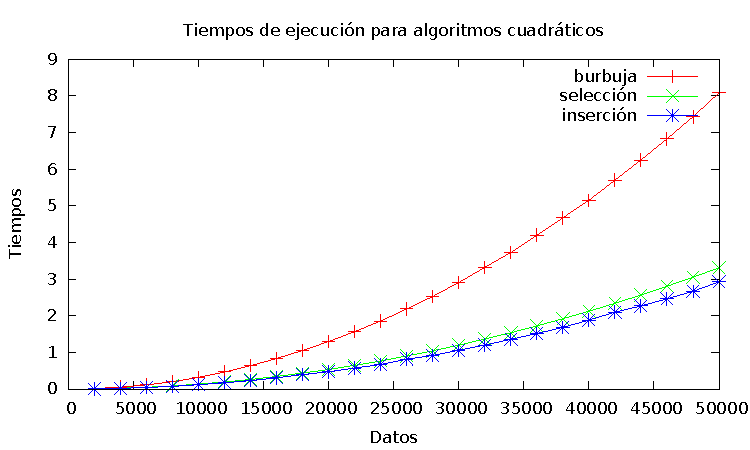
\includegraphics[width=11cm]{comparativa_cuadraticos_g} \centering
	\caption{Algoritmos cuadráticos} \end{figure}

\begin{figure}[H] 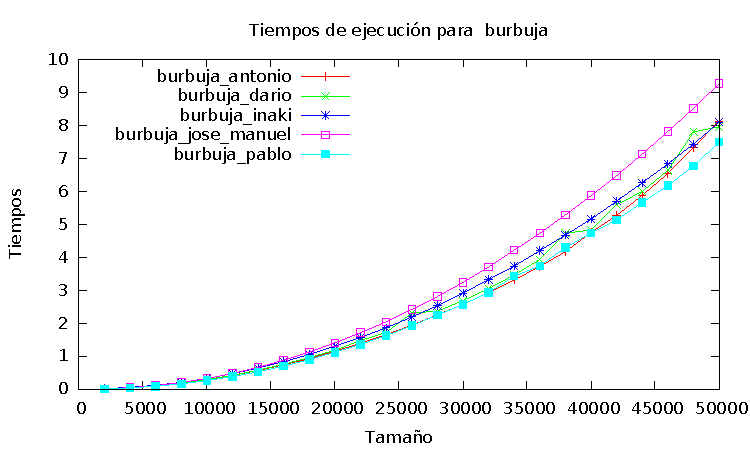
\includegraphics[width=11cm]{burbuja_todos_g} \centering
      \caption{Algoritmo de burbuja} \end{figure}

El algoritmo de la burbuja requiere más del doble de tiempo que cualquiera de los otros dos, que se encuentran casi igualados, teniendo un menor tiempo el de inserción. Probablemente este menor tiempo sea el motivo de que en \textit{quicksort} y \textit{mergesort} se use el algoritmo de inserción para subvectores pequeños.


\begin{figure}[H] 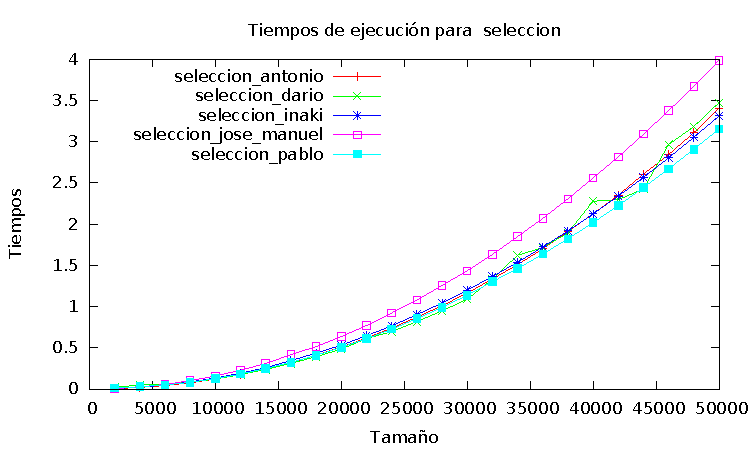
\includegraphics[width=11cm]{seleccion_todos_g} \centering
      \caption{Algoritmo de selección} \end{figure}

\begin{figure}[H] 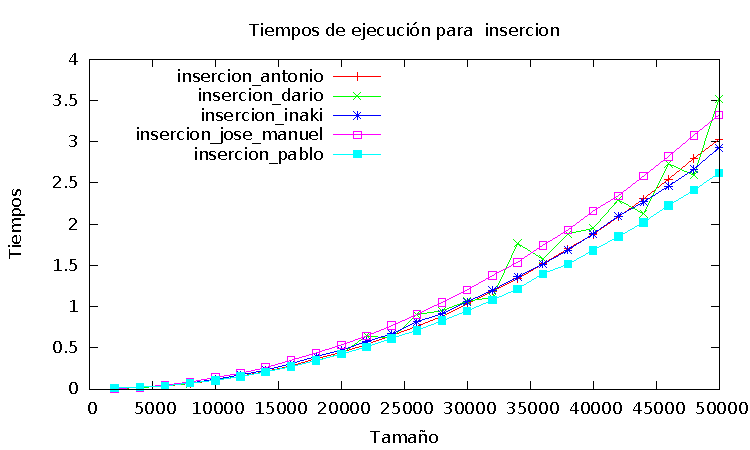
\includegraphics[width=11cm]{insercion_todos_g} \centering
      \caption{Algoritmo de inserción} \end{figure}

\newpage
\subsection{Gráfica de los algoritmos $n\cdot log(n)$ }
\begin{figure}[h] 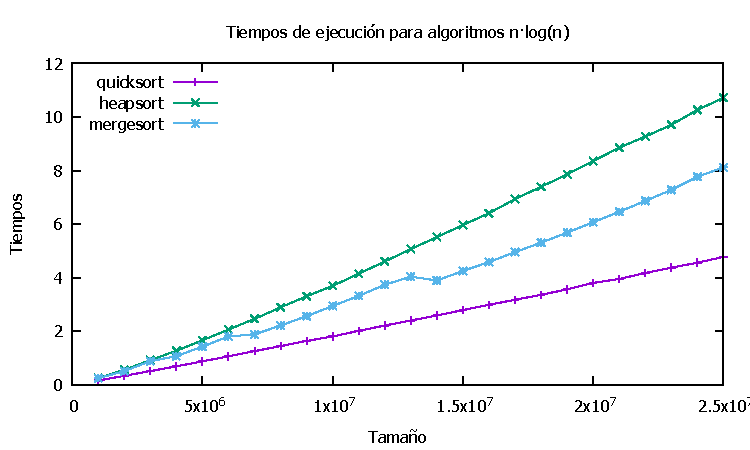
\includegraphics[width=11cm]{comparativa_logaritmicos_g} \centering
	\caption{Algoritmos  $n\cdot log(n)$} \end{figure}

En el algoritmo \textit{mergesort} se aprecian pequeños escalones. Probablemente en cada escalón se incrementa el número de llamadas recursivas, de forma que el tamaño de los subvectores para los que se llama a la función de ordenado por selección (que actúa para tamaños de entrada pequeños) es menor. \\
El algoritmo \textit{quicksort} también usa el algoritmo de inserción por debajo de cierto umbral, pero usa un umbral más pequeño. Esto puede ser la causa de que no presente los escalones.

\begin{figure}[h] 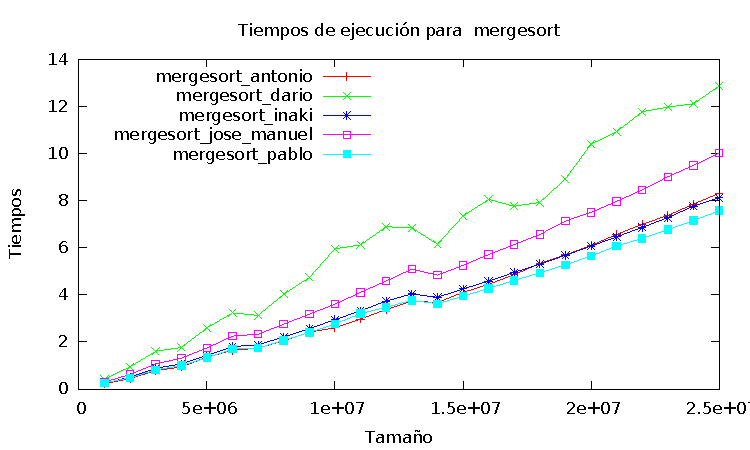
\includegraphics[width=11cm]{mergesort_todos_g} \centering
   \caption{Algoritmo Mergesort} \end{figure}

\begin{figure}[h] 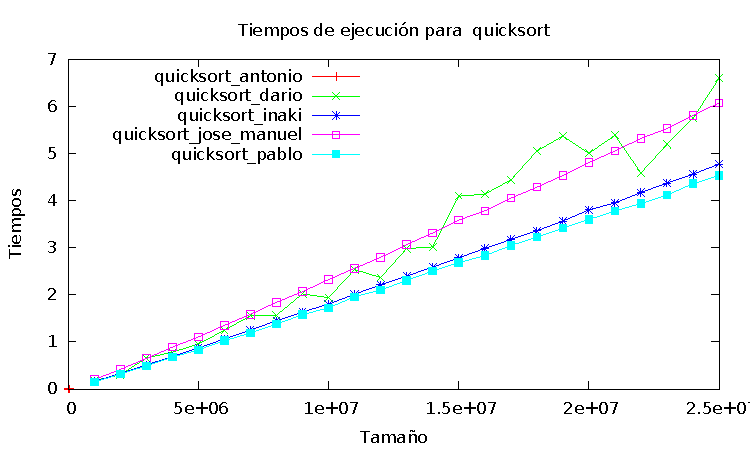
\includegraphics[width=11cm]{quicksort_todos_g} \centering
   \caption{Algoritmo Quicksort} \end{figure}

\begin{figure}[h] 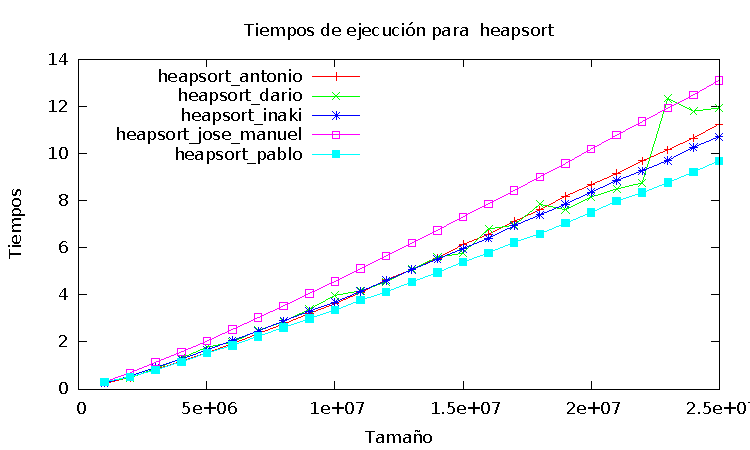
\includegraphics[width=11cm]{heapsort_todos_g} \centering
   \caption{Algoritmo Heapsort} \end{figure}

\newpage

\subsection{Gráfica del algoritmo de Floyd (cúbico)}
\begin{figure}[H] 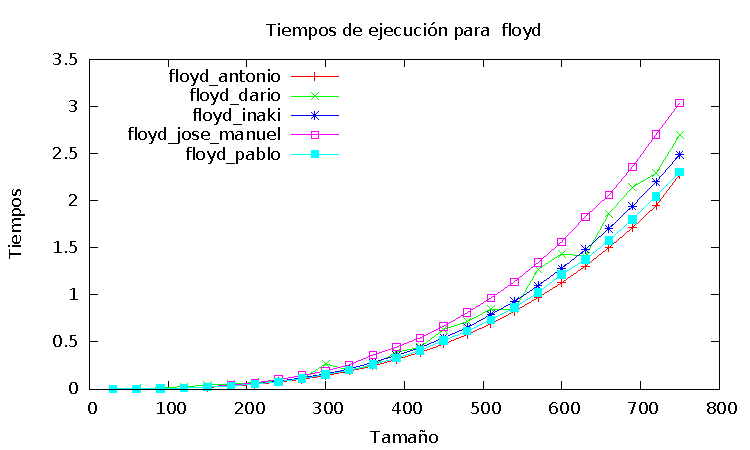
\includegraphics[width=13cm]{floyd_todos_g} \centering
	\caption{Algoritmo de Floyd (cúbico)} \end{figure}

\subsection{Gráfica del algoritmo de Fibonacci $(O(\varphi^n))$}
\begin{figure}[H] 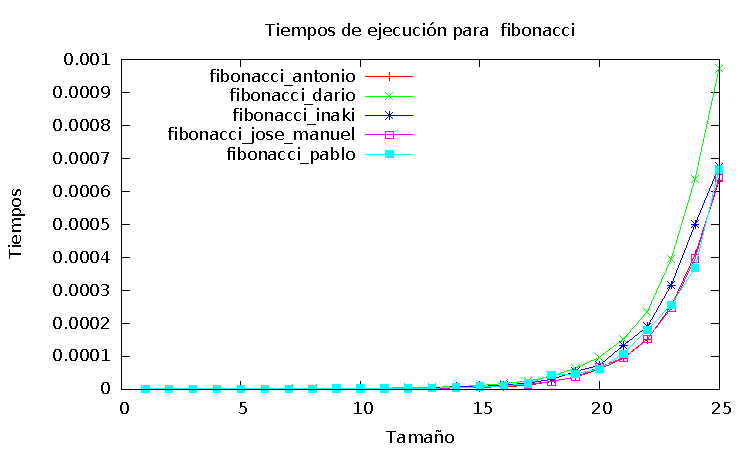
\includegraphics[width=13cm]{fibonacci_todos_g} \centering
	\caption{Algoritmo de Fibonacci} \end{figure}

\subsection{Gráfica del algoritmo de Hanoi ($O(2^n)$)}
\begin{figure}[H] 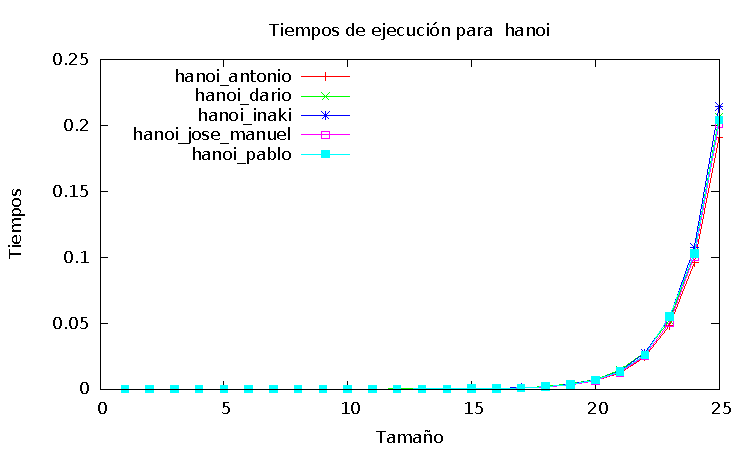
\includegraphics[width=13cm]{hanoi_todos_g} \centering
	\caption{Algoritmo de Hanoi} \end{figure}

\newpage
\subsection{Gráfica de los algoritmos de ordenación}
\begin{figure}[h] 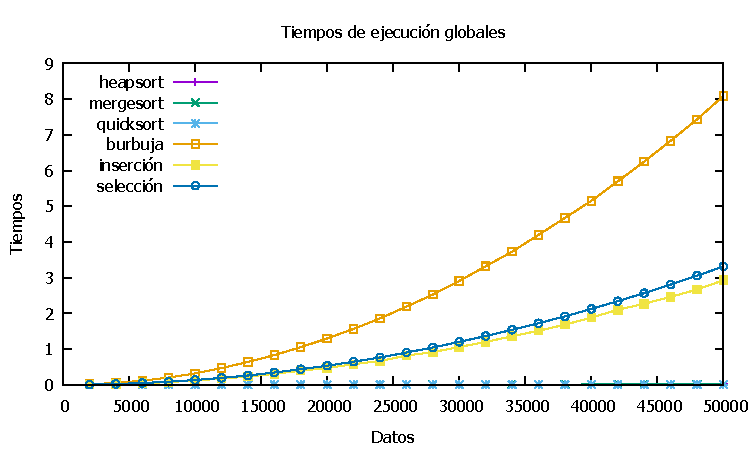
\includegraphics[width=14cm]{comparativa_global_g} \centering
	\caption{Algoritmos de ordenación} \end{figure}

La diferencia en el tiempo de ejecución de los algoritmos de un orden de eficiencia y de otro provoca que los tiempos de los algoritmos de orden de eficiencia $n \cdot \log (n)$ se muestren como una línea horizontal.

\newpage
\section{Ejercicio 3}

\subsection{Eficiencia híbrida de los algoritmos cuadráticos}

\noindent\adjustbox{max width=\textwidth}{%
\begin{tabular}{|l|l|l|l|}
	\hline
	Persona & Burbuja & Inserción & Selección \\
	\hline

	Antonio & $3.67\cdot 10^{-9}n^2 -3.02\cdot 10^{-5}n + 0.189$ ($r=0.99$) & $1.21\cdot 10^{-9}n^2 -5.77\cdot 10^{-6}n + 0,003$ ($r=0.99$) & $1.459 \cdot 10^{-9}n^2 -5.7\cdot 10^{-6}n + 0,002$ ($r=1$) \\
	\hline
  Darío &$89\cdot10^{-3} -1.61671\cdot10^{-5}\cdot n +3\cdot10^{-9}\cdot n^2$ $ (r=0.9999956782)$ &$89 \cdot 10^{-3}+-1.6166\cdot10^{-5} \cdot n +1.68\cdot 10^{-9}\cdot n^2$ $ (r=0.999999728)$&$89\cdot 10^{-3}-1.616\cdot 10^{-5}\cdot n +1.59 \cdot 10^{-9} \cdot n^2$ $(r=0.9996713117)$ \\

   \hline
	José Manuel & $3.85\cdot 10^{-9}n^2 - 7.88\cdot 10^{-6}n + 0.013$ ($r=0.999998565269577$) & $1.32\cdot 10^{-9}n^2 + 4.95\cdot 10^{-7}n - 0.0024$ ($r=0.999979582960209$) & $1.59\cdot 10^{-9}n^2 + 2.93 \cdot 10^{-7} n - 0.0022$ $(r=0.999996280002182)$ \\
   \hline
	Pablo & $3\cdot 10^{-9}n^2 -6\cdot 10^{-6}n + 0,015$ ($r=0.99$) & $10^{-9}n^2 + 4\cdot 10^{-7}n + 0,002$ ($r=0.99$) & $10^{-9}n^2 -2\cdot 10^{-7}n + 0,004$ ($r=1$) \\
	\hline
\end{tabular}
}

\subsection{Eficiencia híbrida de los algoritmos $n \cdot \log(n)$}

\noindent\adjustbox{max width=\textwidth}{
\begin{tabular}{|l|l|l|l|}
	\hline
	Persona & Heapsort & Mergesort & Quicksort \\
	\hline

	Antonio & $2.72 \cdot 10^{-8}n\log(n) -0.55$ ($r=0.999$)  & $1.918 \cdot 10^{-8} n \log(n) - 0.305 $ ($r=0.996$)& $1.06 \cdot 10^{-8}n\log(n) -0.083 $ ($r=0.999$)\\
	\hline
   Darío & $-0.00499364 +2.58544\cdot 10^{-8}\cdot n\cdot log(n) $ $(r=0.999654372) $&$ -0.00499364 +3.0260\cdot 10^{-8}\cdot n\cdot log(x)$ $(r=0.99990783266)$&$-0.00499364  +1.46227\cdot 10^{-8}\cdot n\cdot log(n)$ $(r=0.99994678468)$ \\

   \hline
   José Manuel & $3.13\cdot 10^{-8}n\log(n) - 0.37$ ($r=0.999702622004366$) & $2.29 \cdot 10^{-8}n\log(n) - 0.082$ ($r=0.997798964368601$) & $1.42 \cdot 10^{-8}n\log(n) + 0.020$ ($r=0.999963309603908$)\\
   \hline
	Pablo & $1.8 \cdot 10^{-8}n\log(n) -1.9\cdot 10^{-7}$ ($r=0.995$)  & $2 \cdot 10^{-8} n \log(n) - 1.9\cdot 10^{-7}$ ($r=0.997$)& $1.3 \cdot 10^{-8}n\log(n) -1.9\cdot 10^{-7}$ ($r=0.999$)\\
	\hline

\end{tabular}
}

\subsection{Eficiencia híbrida del algoritmo de Floyd}
\noindent\adjustbox{max width=\textwidth}{
\begin{tabular}{|l|l|l|}
	\hline
	Persona & Eficiencia híbrida de Floyd & Coeficiente de correlación \\
   \hline
 Antonio & $ 6 \cdot 10^{-9}n^3 -7.9 \cdot 10^{-7}n^2 -2.17 \cdot 10^{-4}n +0.012$ & $0.999$ \\
   \hline
 Darío & $ -0.00499364 +0.000217346\cdot n-7.6610\cdot 10^{-7}\cdot n^2 + 6.98242\cdot 10^{-9} \cdot n^3 $ & 0.99999657 \\

   \hline
 José Manuel & $ 6.88 \cdot 10^{-9}n^3 + 2.89 \cdot 10^{-7}n^2 -4.44 \cdot 10^{-5}n +0.001$ & $0.999960701767451$ \\
	\hline
 Pablo & $ 5.1 \cdot 10^{-9}n^3 + 3.8 \cdot 10^{-7}n^2 -8.3 \cdot 10^{-5}n +0.005$ & $1$ \\
 \hline

\end{tabular}
}

\subsection{Eficiencia híbrida del algoritmo de Fibonacci}
\noindent\adjustbox{max width=\textwidth}{
\begin{tabular}{|l|l|l|}

	\hline
	Persona & Eficiencia híbrida de Fibonacci & Coeficiente de correlación \\
	\hline

	Antonio & $3.81 \cdot 10^{-9} \varphi^n +7.21\cdot 10^{-7}$ & $0.999$\\
	\hline
 Darío & $-0.00450426 +0.00150218\cdot\varphi^n $ &0.999987\\

   \hline
 José Manuel & $3.81 \cdot 10^{-9} \varphi^n +9.68\cdot 10^{-7}$ & $0.999939284564366$\\
   \hline
 Pablo & $6.4 \cdot 10^{-9} \varphi^n -1.8\cdot 10^{-8}$ & $0.997$\\
 \hline
\end{tabular}}

\subsection{Eficiencia híbrida del algoritmo de Hanoi}
\noindent\adjustbox{max width=\textwidth}{
\begin{tabular}{|l|l|l|}
	\hline
	Persona & Eficiencia híbrida de Hanoi & Coeficiente de correlación \\
	\hline

	Antonio & $5.69 \cdot 10^{-9} 2^n + 1.1 \cdot 10^{-4}$ & $1$\\
	\hline
 Darío & $ -0.00499364+ 6.37556\cdot 10^{-9}\cdot 2^n$ & 0.983571\\
   \hline
 José Manuel & $6.00 \cdot 10^{-9} 2^n + 9.3 \cdot 10^{-6}$ & $0.999999531007589$\\
   \hline
 Pablo & $6.1 \cdot 10^{-9} 2^n + 1.1 \cdot 10^{-9}$ & $0.9998$\\
 \hline
\end{tabular}}

\newpage
\subsection{Eficiencia hibrida: Comparativa}

Observaremos experimentalmente que si intentamos ajustar los datos de ejecución de los algoritmos con distintas funciones, la que produce un mejor ajuste es la que expresa su eficiencia en el caso medio.

Tomaremos un algoritmo tipo de cada clase de eficiencia y lo intentaremos ajustar mediante distintas curvas.

\vspace{1cm}
\textbf{Algoritmos cuadráticos}

\begin{figure}[H]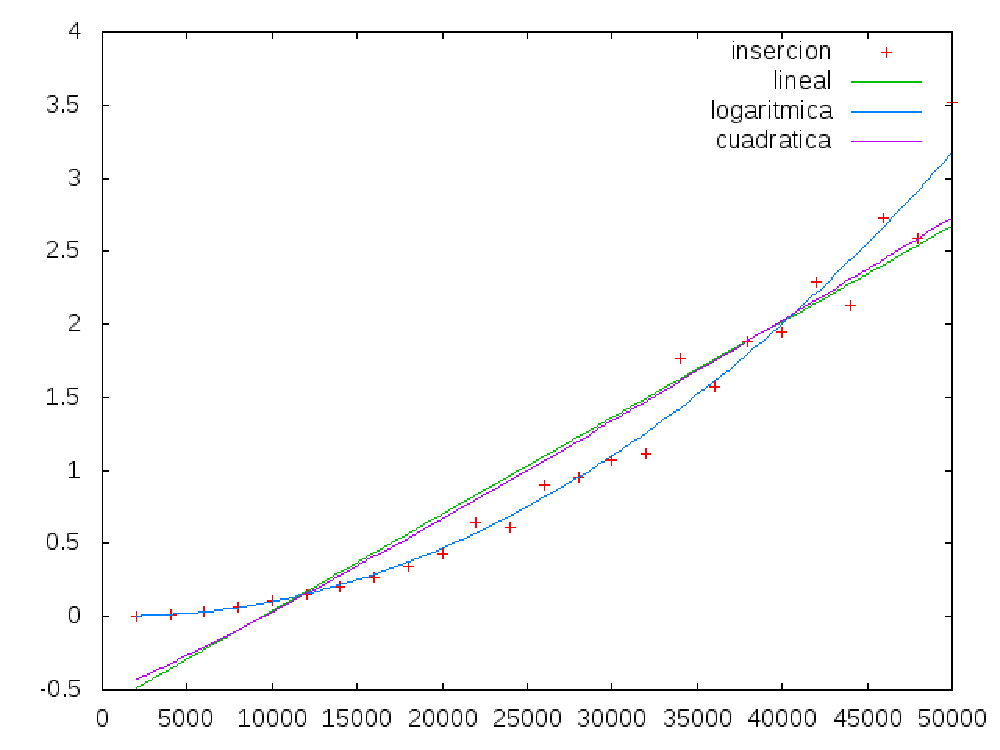
\includegraphics[width=13cm]{img/cuad_hibrida.pdf} \centering
	\caption{Comparativa Cuadráticos Híbrida}\end{figure}

Como vemos la función cuadrática es la que mejor se ajusta a los datos.

\vspace{1cm}

\textbf{Algoritmos logarítmicos}

Vamos a aproximar los datos del \textit{quicksort} con una función lineal y una logarítmica. Veremos que la aproximación lineal es mejor de lo que de primeras podríamos pensar.


\begin{figure}[H]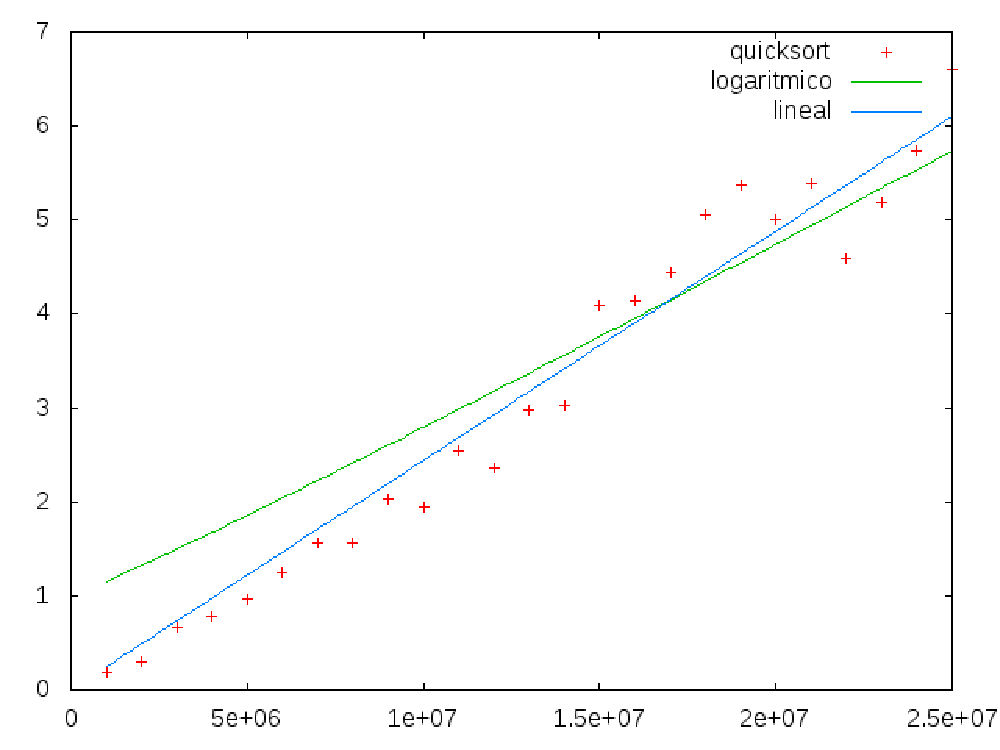
\includegraphics[width=13cm]{img/log_hibrida.pdf} \centering
	\caption{Comparativa Logarítmica Híbrida}\end{figure}

Esto se debe a que el logaritmo es menor que cualquier raiz, asintóticamente; es por esto que la función O(nlog(n)) se comporta de una manera parecida a una lineal.


\vspace{1cm}

\textbf{Algoritmos Exponenciales}

Ejecutaremos el algoritmo de Hanói y lo compararemos con funciones polinómicas de diverso grado.

\begin{figure}[H]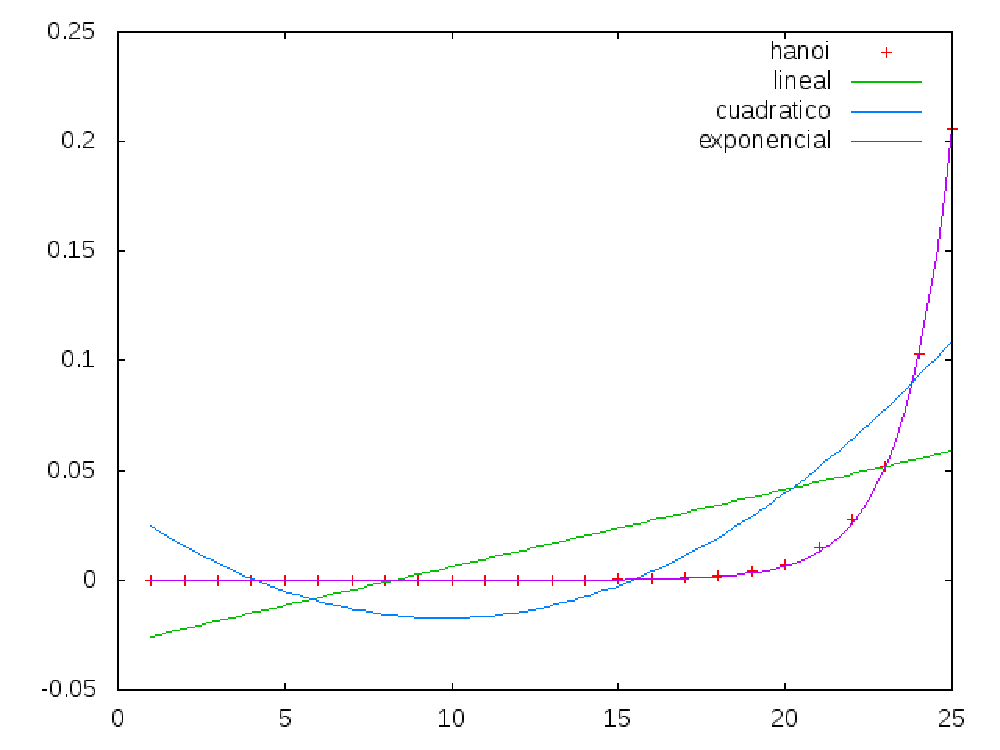
\includegraphics[width=13cm]{img/expo_hibrida2.pdf} \centering
	\caption{Comparativa Exponencial Híbrida}\end{figure}

Como era de esperar aproximar el crecimiento exponencial mediante funciones polinómicas es inviable. Cabe destacar que no empleamos algoritmos cúbicos porque el método de mínimos cuadrados devuelve una aproximación tan nefasta que se dejan de apreciar bien las demás funciones en la gráfica.

\vspace{1cm}

\textbf{Algoritmos Cúbicos}

Por último aproximaremos mediante las funciones que ya hemos tratado los datos resultantes de la ejecución del algoritmo cúbico de Floyd.

\begin{figure}[H]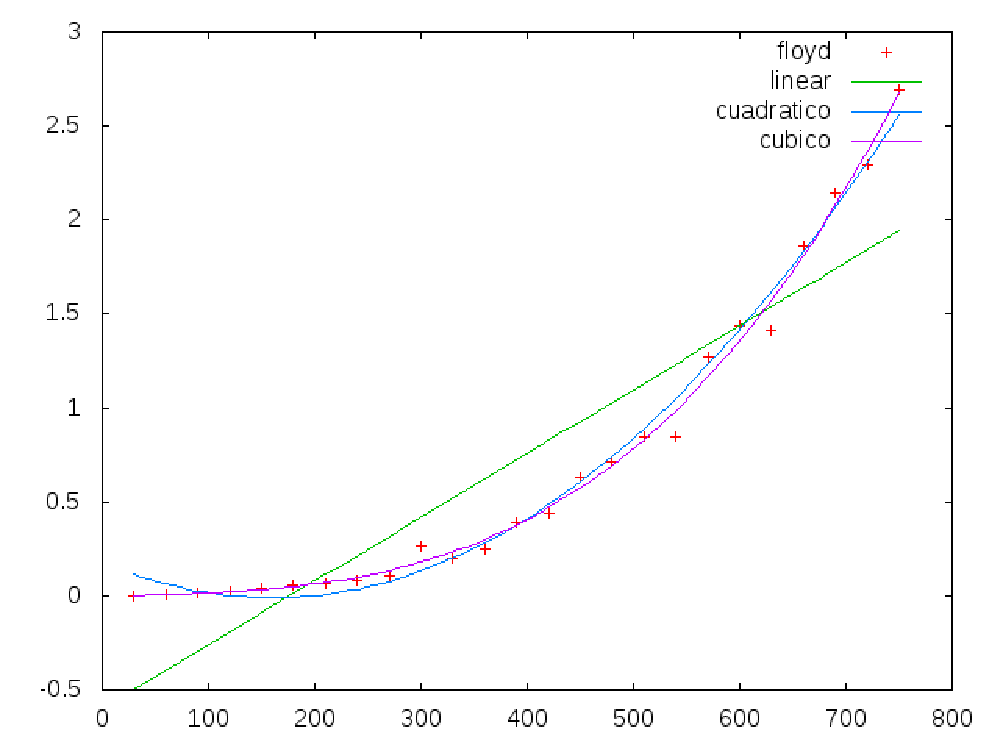
\includegraphics[width=13cm]{img/floyd_hibrida.pdf} \centering
	\caption{Comparativa Floyd Híbrida}\end{figure}

\begin{framed}
	Se ha de notar que no hemos intentado ajustar el algoritmo de floyd con una función exponencial. Esto se debe a que dicho ajuste es tan poco realista que las constantes se salen del rango de precisión aritmética del programa empleado para el su cálculo.(gnuplot)
\end{framed}


Por último queremos comentar la proximidad de las funciones cuadrática y cúbica, salvo para datos pequeños que ajusta mejor la cúbica; esto se debe a que las constantes difieren mucho y los datos son insuficientes, por tanto, en un pequeño intervalo las funciones pueden llegar a "parecerse".

\newpage
\section{Ejercicio 4}
\subsection{Optimización de Burbuja}
\begin{tabular}{|l|l|l|l|l|}
	\hline
	Tamaño & O0 & O1 & O2 & O3 \\
	\hline
	\hline
	2000 & 0,011413 & 0,00767027 & 0,00729825 & 0,00886811 \\
	\hline
	4000 & 0,0453449 & 0,0174315 & 0,0176928 & 0,0188218 \\
	\hline
	6000 & 0,101489 & 0,0384904 & 0,0332072 & 0,0414915 \\
	\hline
	8000 & 0,181023 & 0,073721 & 0,0650689 & 0,0724921 \\
	\hline
	10000 & 0,285049 & 0,124228 & 0,109425 & 0,10953 \\
	\hline
	12000 & 0,412749 & 0,18656 & 0,163998 & 0,16372 \\
	\hline
	14000 & 0,564313 & 0,262641 & 0,230543 & 0,230014 \\
	\hline
	16000 & 0,736274 & 0,351798 & 0,308667 & 0,307852 \\
	\hline
	18000 & 0,9231 & 0,450813 & 0,402396 & 0,400231 \\
	\hline
	20000 & 1,14936 & 0,566283 & 0,496466 & 0,495054 \\
	\hline
	22000 & 1,38726 & 0,692367 & 0,608456 & 0,609754 \\
	\hline
	24000 & 1,64832 & 0,830683 & 0,736194 & 0,729921 \\
	\hline
	26000 & 1,93603 & 0,983933 & 0,869556 & 0,865144 \\
	\hline
	28000 & 2,24947 & 1,15135 & 1,00542 & 1,01213 \\
	\hline
	30000 & 2,56848 & 1,33711 & 1,16349 & 1,16509 \\
	\hline
	32000 & 2,92343 & 1,53865 & 1,33626 & 1,33301 \\
	\hline
	34000 & 3,31074 & 1,74399 & 1,51139 & 1,51782 \\
	\hline
	36000 & 3,71294 & 1,95579 & 1,70749 & 1,71322 \\
	\hline
	38000 & 4,16954 & 2,19283 & 1,89924 & 1,93158 \\
	\hline
	40000 & 4,74451 & 2,44766 & 2,11777 & 2,1556 \\
	\hline
	42000 & 5,26566 & 2,70633 & 2,3327 & 2,40839 \\
	\hline
	44000 & 5,87307 & 2,97798 & 2,56785 & 2,70971 \\
	\hline
	46000 & 6,53502 & 3,25714 & 2,82431 & 3,00307 \\
	\hline
	48000 & 7,32794 & 3,5752 & 3,0812 & 3,29677 \\
	\hline
	50000 & 8,1269 & 3,92439 & 3,36591 & 3,64032 \\
	\hline
\end{tabular}

\begin{figure}[H]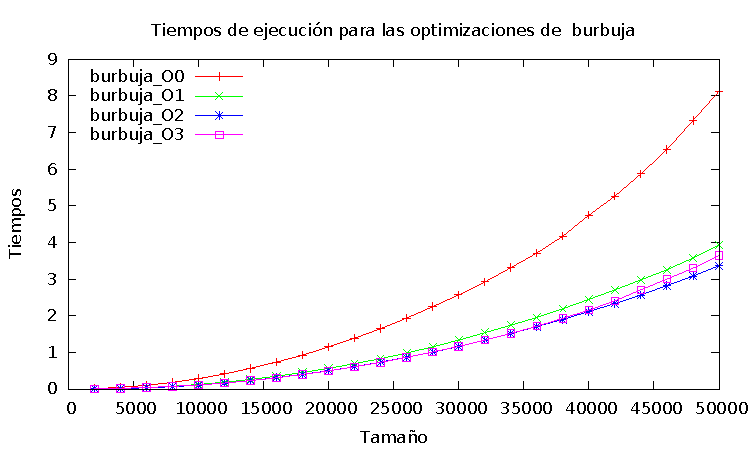
\includegraphics[width=13cm]{img/burbuja_optim_g.pdf} \centering
	\caption{Optimización Burbuja}\end{figure}

\subsection{Optimización de Selección}
\begin{tabular}{|l|l|l|l|l|}
	\hline
	Tamaño & O0 & O1 & O2 & O3 \\
	\hline
	\hline
	2000 & 0,00515467 & 0,00518568 & 0,00295874 & 0,00781173 \\
	\hline
	4000 & 0,019939 & 0,014322 & 0,0105633 & 0,0231289 \\
	\hline
	6000 & 0,0433264 & 0,0220253 & 0,0143769 & 0,0405819 \\
	\hline
	8000 & 0,0764116 & 0,0337371 & 0,0226186 & 0,0421702 \\
	\hline
	10000 & 0,121217 & 0,0446664 & 0,0325282 & 0,0535996 \\
	\hline
	12000 & 0,177811 & 0,0540817 & 0,0428159 & 0,0716839 \\
	\hline
	14000 & 0,244628 & 0,0645687 & 0,0581941 & 0,0972 \\
	\hline
	16000 & 0,320919 & 0,0764816 & 0,0755991 & 0,127552 \\
	\hline
	18000 & 0,410265 & 0,0952006 & 0,0954893 & 0,162643 \\
	\hline
	20000 & 0,509134 & 0,117962 & 0,117173 & 0,202739 \\
	\hline
	22000 & 0,61807 & 0,142821 & 0,142361 & 0,248662 \\
	\hline
	24000 & 0,739096 & 0,170087 & 0,168087 & 0,29886 \\
	\hline
	26000 & 0,872412 & 0,202472 & 0,197149 & 0,347695 \\
	\hline
	28000 & 1,01093 & 0,236475 & 0,232414 & 0,403681 \\
	\hline
	30000 & 1,16345 & 0,26976 & 0,271271 & 0,466755 \\
	\hline
	32000 & 1,33592 & 0,308442 & 0,298858 & 0,530757 \\
	\hline
	34000 & 1,50895 & 0,347973 & 0,335636 & 0,602817 \\
	\hline
	36000 & 1,70088 & 0,39664 & 0,378081 & 0,676565 \\
	\hline
	38000 & 1,91222 & 0,438568 & 0,418638 & 0,753679 \\
	\hline
	40000 & 2,12327 & 0,485922 & 0,467527 & 0,836347 \\
	\hline
	42000 & 2,35229 & 0,538412 & 0,513721 & 0,930382 \\
	\hline
	44000 & 2,60759 & 0,591486 & 0,561665 & 1,02398 \\
	\hline
	46000 & 2,8435 & 0,645382 & 0,613942 & 1,12764 \\
	\hline
	48000 & 3,11111 & 0,706955 & 0,668329 & 1,23934 \\
	\hline
	50000 & 3,40647 & 0,766349 & 0,725693 & 1,3503 \\
	\hline
\end{tabular}

\begin{figure}[H]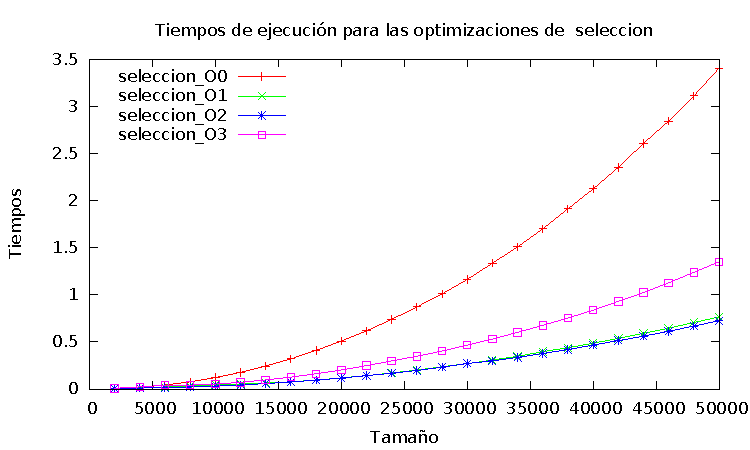
\includegraphics[width=13cm]{img/seleccion_optim_g.pdf} \centering
	\caption{Optimización Selección}\end{figure}

\subsection{Optimización de Inserción}
\begin{tabular}{|l|l|l|l|l|}
	\hline
	Tamaño & O0 & O1 & O2 & O3 \\
	\hline
	\hline
	2000 & 0,0044917 & 0,00195844 & 0,00468466 & 0,00632375 \\
	\hline
	4000 & 0,0186884 & 0,00730802 & 0,011605 & 0,0158228 \\
	\hline
	6000 & 0,0377812 & 0,0137966 & 0,0194001 & 0,0252668 \\
	\hline
	8000 & 0,0669812 & 0,0233589 & 0,0324477 & 0,0403882 \\
	\hline
	10000 & 0,107932 & 0,037316 & 0,0457049 & 0,0458144 \\
	\hline
	12000 & 0,154884 & 0,0521311 & 0,0622211 & 0,0609401 \\
	\hline
	14000 & 0,213453 & 0,0710041 & 0,0841461 & 0,0828928 \\
	\hline
	16000 & 0,280269 & 0,0935783 & 0,10946 & 0,108517 \\
	\hline
	18000 & 0,368311 & 0,120639 & 0,138311 & 0,137761 \\
	\hline
	20000 & 0,443013 & 0,150077 & 0,173783 & 0,168523 \\
	\hline
	22000 & 0,541246 & 0,181517 & 0,21135 & 0,206084 \\
	\hline
	24000 & 0,649446 & 0,217471 & 0,263303 & 0,248386 \\
	\hline
	26000 & 0,760331 & 0,257764 & 0,301838 & 0,295198 \\
	\hline
	28000 & 0,882182 & 0,282926 & 0,34644 & 0,335562 \\
	\hline
	30000 & 1,03487 & 0,336947 & 0,390829 & 0,383697 \\
	\hline
	32000 & 1,18717 & 0,390892 & 0,452143 & 0,438392 \\
	\hline
	34000 & 1,33726 & 0,444824 & 0,492365 & 0,497819 \\
	\hline
	36000 & 1,51744 & 0,500244 & 0,552547 & 0,557171 \\
	\hline
	38000 & 1,70203 & 0,557174 & 0,613258 & 0,624803 \\
	\hline
	40000 & 1,87561 & 0,613763 & 0,683716 & 0,696917 \\
	\hline
	42000 & 2,08887 & 0,679748 & 0,747116 & 0,773843 \\
	\hline
	44000 & 2,30682 & 0,746035 & 0,821289 & 0,846906 \\
	\hline
	46000 & 2,54603 & 0,820299 & 0,895795 & 0,927429 \\
	\hline
	48000 & 2,79809 & 0,891268 & 0,976704 & 1,02405 \\
	\hline
	50000 & 3,02904 & 0,987499 & 1,05693 & 1,11367 \\
	\hline
\end{tabular}

\begin{figure}[H]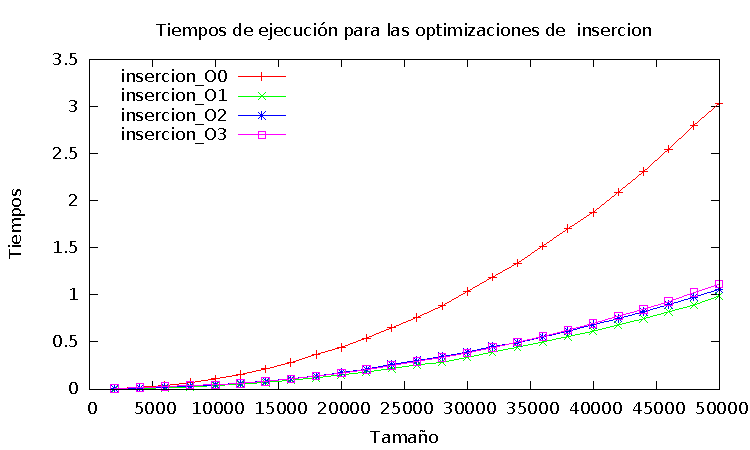
\includegraphics[width=13cm]{img/insercion_optim_g.pdf} \centering
	\caption{Optimización Inserción}\end{figure}

\subsection{Optimización de Quicksort}
\begin{tabular}{|l|l|l|l|l|}
	\hline
	Tamaño & O0 & O1 & O2 & O3 \\
	\hline
	\hline
	1000000 & 0,140354 & 0,108984 & 0,0723194 & 0,145934 \\
	\hline
	2000000 & 0,290671 & 0,156802 & 0,160161 & 0,149131 \\
	\hline
	3000000 & 0,451042 & 0,246713 & 0,254127 & 0,234554 \\
	\hline
	4000000 & 0,609228 & 0,342867 & 0,349069 & 0,318788 \\
	\hline
	5000000 & 0,768809 & 0,4443 & 0,444097 & 0,413716 \\
	\hline
	6000000 & 0,939232 & 0,538326 & 0,544886 & 0,492602 \\
	\hline
	7000000 & 1,09785 & 0,63253 & 0,631983 & 0,581733 \\
	\hline
	8000000 & 1,26473 & 0,666134 & 0,742487 & 0,674327 \\
	\hline
	9000000 & 1,43536 & 0,744798 & 0,842272 & 0,768711 \\
	\hline
	10000000 & 1,62045 & 0,826848 & 0,941442 & 0,854967 \\
	\hline
	11000000 & 1,79408 & 0,928571 & 1,03906 & 0,95514 \\
	\hline
	12000000 & 1,95441 & 1,01002 & 1,14623 & 1,0418 \\
	\hline
	13000000 & 2,12925 & 1,11231 & 1,2527 & 1,15554 \\
	\hline
	14000000 & 2,30318 & 1,22047 & 1,35309 & 1,24338 \\
	\hline
	15000000 & 2,45234 & 1,49 & 1,45845 & 1,34034 \\
	\hline
	16000000 & 2,62369 & 1,5982 & 1,54854 & 1,44701 \\
	\hline
	17000000 & 2,81701 & 1,70221 & 1,69107 & 1,52156 \\
	\hline
	18000000 & 3,02744 & 1,81955 & 1,76673 & 1,60615 \\
	\hline
	19000000 & 3,26244 & 1,94608 & 1,89436 & 1,74194 \\
	\hline
	20000000 & 3,44172 & 2,06746 & 2,01535 & 1,84022 \\
	\hline
	21000000 & 3,69781 & 2,17781 & 2,11261 & 1,8951 \\
	\hline
	22000000 & 3,94126 & 1,99071 & 2,23865 & 2,03436 \\
	\hline
	23000000 & 4,20059 & 2,0863 & 2,38896 & 2,12836 \\
	\hline
	24000000 & 4,36635 & 2,53774 & 2,49616 & 2,24849 \\
	\hline
	25000000 & 4,59738 & 2,68214 & 2,59766 & 2,34848 \\
	\hline
\end{tabular}

\begin{figure}[H]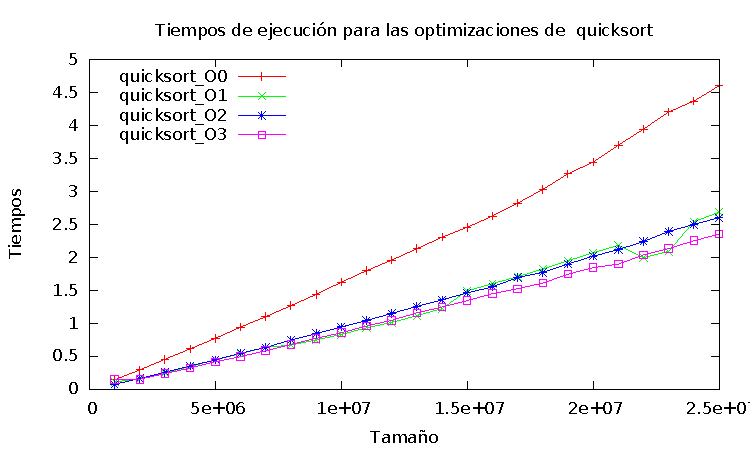
\includegraphics[width=13cm]{img/quicksort_optim_g.pdf} \centering
	\caption{Optimización Quicksort}\end{figure}

\subsection{Optimización de Mergesort}
\begin{tabular}{|l|l|l|l|l|}
	\hline
	Tamano & O0 & O1 & O2 & O3 \\
	\hline
	\hline
	1000000 & 0,217543 & 0,14913 & 0,155871 & 0,142481 \\
	\hline
	2000000 & 0,453951 & 0,222821 & 0,216717 & 0,200155 \\
	\hline
	3000000 & 0,782204 & 0,36456 & 0,376277 & 0,397549 \\
	\hline
	4000000 & 0,942283 & 0,467165 & 0,479917 & 0,506261 \\
	\hline
	5000000 & 1,35111 & 0,605842 & 0,626561 & 0,673165 \\
	\hline
	6000000 & 1,64402 & 0,768339 & 0,792216 & 0,848724 \\
	\hline
	7000000 & 1,73735 & 0,83704 & 0,851907 & 0,897172 \\
	\hline
	8000000 & 2,05693 & 0,979482 & 0,99871 & 1,05081 \\
	\hline
	9000000 & 2,41358 & 1,12709 & 1,15498 & 1,21198 \\
	\hline
	10000000 & 2,59924 & 1,28209 & 1,33451 & 1,39942 \\
	\hline
	11000000 & 2,97113 & 1,45494 & 1,51848 & 1,33572 \\
	\hline
	12000000 & 3,37961 & 1,62648 & 1,70929 & 1,52628 \\
	\hline
	13000000 & 3,73061 & 1,76984 & 1,86878 & 1,66805 \\
	\hline
	14000000 & 3,67511 & 1,78486 & 1,85468 & 1,64051 \\
	\hline
	15000000 & 4,10348 & 1,94386 & 2,01848 & 2,07944 \\
	\hline
	16000000 & 4,44356 & 2,1014 & 2,18132 & 2,23598 \\
	\hline
	17000000 & 4,85593 & 2,28211 & 2,35156 & 2,44318 \\
	\hline
	18000000 & 5,33545 & 2,45917 & 2,5384 & 2,20835 \\
	\hline
	19000000 & 5,69309 & 2,64892 & 2,7174 & 2,3847 \\
	\hline
	20000000 & 6,09616 & 2,82851 & 2,91747 & 2,58527 \\
	\hline
	21000000 & 6,56725 & 3,00782 & 3,05882 & 2,74309 \\
	\hline
	22000000 & 6,99638 & 3,17541 & 3,27018 & 2,90998 \\
	\hline
	23000000 & 7,37357 & 3,35114 & 3,45721 & 3,10196 \\
	\hline
	24000000 & 7,85359 & 3,58095 & 3,68085 & 3,27219 \\
	\hline
	25000000 & 8,30719 & 3,76735 & 3,90997 & 4,03064 \\
	\hline
\end{tabular}

\begin{figure}[H]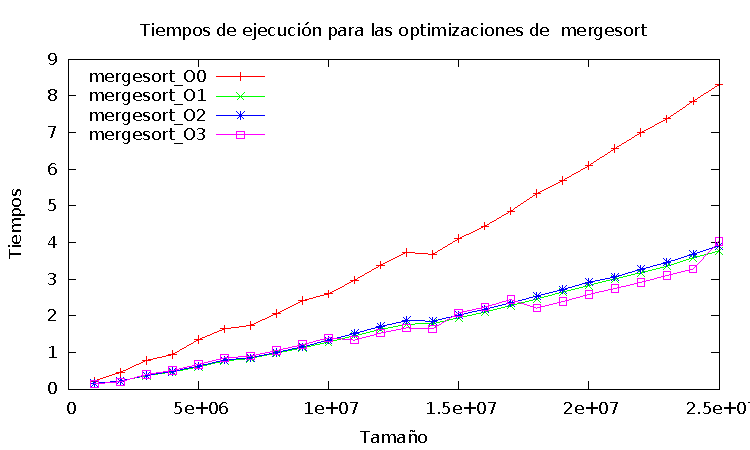
\includegraphics[width=13cm]{img/mergesort_optim_g.pdf} \centering
	\caption{Optimización Mergesort}\end{figure}

\subsection{Optimización de Heapsort}
\begin{tabular}{|l|l|l|l|l|}
	\hline
	Tamaño & O0 & O1 & O2 & O3 \\
	\hline
	\hline
	1000000 & 0,22421 & 0,162612 & 0,189088 & 0,124874 \\
	\hline
	2000000 & 0,500762 & 0,273371 & 0,244746 & 0,241887 \\
	\hline
	3000000 & 0,833796 & 0,481102 & 0,409636 & 0,415654 \\
	\hline
	4000000 & 1,17323 & 0,7742 & 0,610973 & 0,607138 \\
	\hline
	5000000 & 1,54404 & 0,996273 & 0,776043 & 0,797603 \\
	\hline
	6000000 & 1,9243 & 1,37394 & 0,985671 & 1,00536 \\
	\hline
	7000000 & 2,35331 & 1,64974 & 1,20662 & 1,18956 \\
	\hline
	8000000 & 2,76399 & 2,12896 & 1,4108 & 1,39054 \\
	\hline
	9000000 & 3,20945 & 2,41538 & 1,59403 & 1,65914 \\
	\hline
	10000000 & 3,62159 & 2,84488 & 1,84175 & 1,8471 \\
	\hline
	11000000 & 4,09924 & 3,23755 & 2,06092 & 2,05358 \\
	\hline
	12000000 & 4,63249 & 3,64295 & 2,29729 & 2,30546 \\
	\hline
	13000000 & 5,0709 & 4,02955 & 2,52116 & 2,54731 \\
	\hline
	14000000 & 5,55749 & 4,49345 & 2,76215 & 2,79191 \\
	\hline
	15000000 & 6,13142 & 4,81149 & 3,06052 & 3,02149 \\
	\hline
	16000000 & 6,57542 & 5,38016 & 3,32291 & 3,27649 \\
	\hline
	17000000 & 7,11513 & 5,97832 & 3,9232 & 3,5468 \\
	\hline
	18000000 & 7,60767 & 6,24962 & 4,19137 & 3,80012 \\
	\hline
	19000000 & 8,18748 & 6,70817 & 4,43557 & 4,11741 \\
	\hline
	20000000 & 8,6704 & 7,25184 & 4,95784 & 4,41006 \\
	\hline
	21000000 & 9,14739 & 7,9527 & 4,99053 & 4,66293 \\
	\hline
	22000000 & 9,68533 & 7,96672 & 5,24068 & 4,98344 \\
	\hline
	23000000 & 10,1561 & 8,50889 & 5,59346 & 5,2685 \\
	\hline
	24000000 & 10,6587 & 9,2256 & 5,93449 & 5,72653 \\
	\hline
	25000000 & 11,2477 & 9,74256 & 6,22192 & 5,78521 \\
	\hline
\end{tabular}

\begin{figure}[H]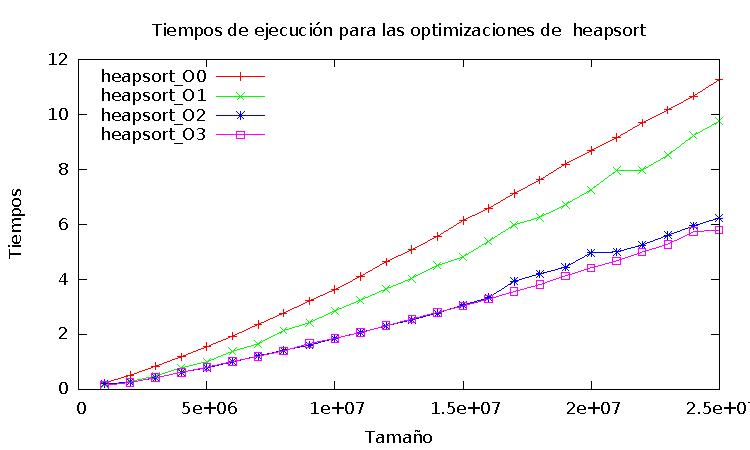
\includegraphics[width=13cm]{img/heapsort_optim_g.pdf} \centering
	\caption{Optimización Heapsort}\end{figure}

\subsection{Optimización de Floyd}
\begin{tabular}{|l|l|l|l|l|}
	\hline
	Tamaño & O0 & O1 & O2 & O3 \\
	\hline
	\hline
	30 & 0,000224592 & 0,00011651 & 5,3519e-05 & 8,2696e-05 \\
	\hline
	60 & 0,00139668 & 0,000824097 & 0,000434777 & 0,00066088 \\
	\hline
	90 & 0,00455954 & 0,00221353 & 0,00143882 & 0,0017947 \\
	\hline
	120 & 0,0097123 & 0,00552435 & 0,00333 & 0,003445 \\
	\hline
	150 & 0,0186866 & 0,00662406 & 0,00634183 & 0,00455262 \\
	\hline
	180 & 0,0314451 & 0,0111573 & 0,00524036 & 0,00537472 \\
	\hline
	210 & 0,0493398 & 0,0161588 & 0,0079134 & 0,00841322 \\
	\hline
	240 & 0,0735784 & 0,0223456 & 0,0118256 & 0,0121501 \\
	\hline
	270 & 0,104221 & 0,029449 & 0,0166624 & 0,0174797 \\
	\hline
	300 & 0,142323 & 0,0374595 & 0,0227272 & 0,0226334 \\
	\hline
	330 & 0,189639 & 0,04001 & 0,0301813 & 0,0301163 \\
	\hline
	360 & 0,244835 & 0,0530836 & 0,0393631 & 0,0403175 \\
	\hline
	390 & 0,314773 & 0,0663636 & 0,052403 & 0,0504283 \\
	\hline
	420 & 0,38828 & 0,0816097 & 0,0615897 & 0,0625458 \\
	\hline
	450 & 0,477007 & 0,0991475 & 0,0802832 & 0,0778467 \\
	\hline
	480 & 0,579336 & 0,121864 & 0,0910224 & 0,0951062 \\
	\hline
	510 & 0,692464 & 0,14376 & 0,114807 & 0,115598 \\
	\hline
	540 & 0,824832 & 0,169778 & 0,128893 & 0,136475 \\
	\hline
	570 & 0,970557 & 0,201297 & 0,151532 & 0,161607 \\
	\hline
	600 & 1,12768 & 0,243252 & 0,17859 & 0,192296 \\
	\hline
	630 & 1,30571 & 0,269596 & 0,207239 & 0,227301 \\
	\hline
	660 & 1,50015 & 0,309459 & 0,236404 & 0,252319 \\
	\hline
	690 & 1,71206 & 0,355785 & 0,271002 & 0,288827 \\
	\hline
	720 & 1,94615 & 0,402889 & 0,309074 & 0,328996 \\
	\hline
	750 & 2,27876 & 0,456356 & 0,349434 & 0,374203 \\
	\hline
\end{tabular}

\begin{figure}[H]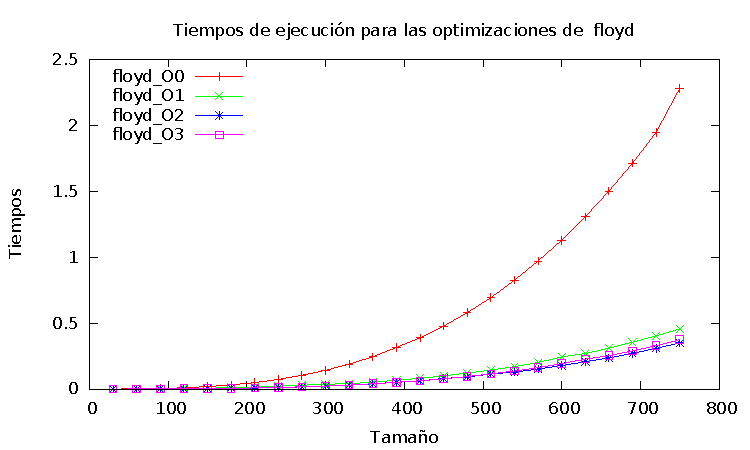
\includegraphics[width=13cm]{img/floyd_optim_g.pdf} \centering
	\caption{Optimización Floyd}\end{figure}

\subsection{Optimización de Fibonacci}
\begin{tabular}{|l|l|l|l|l|}
	\hline
	Tamano & O0 & O1 & O2 & O3 \\
	\hline
	\hline
	1 & 1,44e-07 & 3,74e-07 & 4,1e-07 & 4,05e-07 \\
	\hline
	2 & 1,66e-07 & 4,1e-07 & 3,73e-07 & 3,28e-07 \\
	\hline
	3 & 1,68e-07 & 4,14e-07 & 4,09e-07 & 2,58e-07 \\
	\hline
	4 & 2,13e-07 & 4,04e-07 & 4,34e-07 & 3,41e-07 \\
	\hline
	5 & 3,51e-07 & 6,09e-07 & 4,66e-07 & 3,84e-07 \\
	\hline
	6 & 2,56e-07 & 4,69e-07 & 5,09e-07 & 3,21e-07 \\
	\hline
	7 & 4,33e-07 & 6,5e-07 & 6,21e-07 & 4,85e-07 \\
	\hline
	8 & 6,82e-07 & 6,61e-07 & 7,88e-07 & 6,11e-07 \\
	\hline
	9 & 8,29e-07 & 1,177e-06 & 9,62e-07 & 7,74e-07 \\
	\hline
	10 & 1,129e-06 & 1,279e-06 & 1,214e-06 & 1e-06 \\
	\hline
	11 & 1,508e-06 & 1,748e-06 & 1,417e-06 & 8,91e-07 \\
	\hline
	12 & 2,103e-06 & 2,173e-06 & 1,901e-06 & 1,345e-06 \\
	\hline
	13 & 2,937e-06 & 3,159e-06 & 2,467e-06 & 2,21e-06 \\
	\hline
	14 & 4,122e-06 & 4,288e-06 & 3,647e-06 & 3,337e-06 \\
	\hline
	15 & 5,257e-06 & 6,368e-06 & 5,443e-06 & 4,03e-06 \\
	\hline
	16 & 7,144e-06 & 9,167e-06 & 7,527e-06 & 5,865e-06 \\
	\hline
	17 & 1,1107e-05 & 1,4243e-05 & 1,1615e-05 & 8,258e-06 \\
	\hline
	18 & 2,3568e-05 & 2,2602e-05 & 1,8075e-05 & 1,298e-05 \\
	\hline
	19 & 3,6087e-05 & 3,5879e-05 & 2,8786e-05 & 1,6151e-05 \\
	\hline
	20 & 6,0297e-05 & 5,7232e-05 & 4,3465e-05 & 2,8727e-05 \\
	\hline
	21 & 9,3336e-05 & 9,188e-05 & 7,0517e-05 & 4,4614e-05 \\
	\hline
	22 & 0,000150115 & 0,000148022 & 8,5657e-05 & 6,9375e-05 \\
	\hline
	23 & 0,000252328 & 0,000238767 & 0,00013781 & 0,00011195 \\
	\hline
	24 & 0,000407404 & 0,000366446 & 0,000223523 & 0,00017296 \\
	\hline
	25 & 0,000630981 & 0,000592224 & 0,000359381 & 0,000286624 \\
	\hline
\end{tabular}

\begin{figure}[H]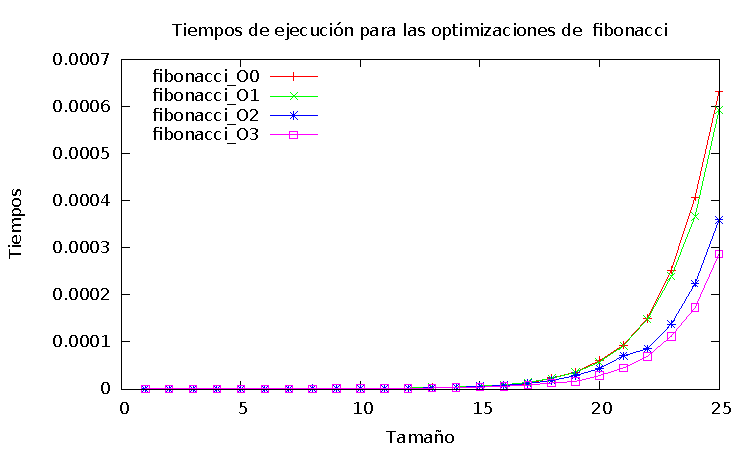
\includegraphics[width=13cm]{img/fibonacci_optim_g.pdf} \centering
	\caption{Optimización Fibonacci}\end{figure}

\subsection{Optimización de Hanói}
\begin{tabular}{|l|l|l|l|l|}
	\hline
	Tamano & O0 & O1 & O2 & O3 \\
	\hline
	\hline
	1 & 1,79e-07 & 2,03e-07 & 3,96e-07 & 3,6e-07 \\
	\hline
	2 & 2,04e-07 & 3,01e-07 & 6,21e-07 & 5,05e-07 \\
	\hline
	3 & 2,85e-07 & 3,43e-07 & 6,5e-07 & 4,77e-07 \\
	\hline
	4 & 4,31e-07 & 3,5e-07 & 9,66e-07 & 6,56e-07 \\
	\hline
	5 & 6,54e-07 & 4,43e-07 & 1,256e-06 & 6,19e-07 \\
	\hline
	6 & 9,35e-07 & 6,41e-07 & 1,636e-06 & 9,81e-07 \\
	\hline
	7 & 1,491e-06 & 9,51e-07 & 2,128e-06 & 1,641e-06 \\
	\hline
	8 & 2,662e-06 & 1,447e-06 & 2,964e-06 & 2,851e-06 \\
	\hline
	9 & 4,721e-06 & 2,48e-06 & 4,946e-06 & 3,05e-06 \\
	\hline
	10 & 8,768e-06 & 4,672e-06 & 8,532e-06 & 5,089e-06 \\
	\hline
	11 & 1,7136e-05 & 8,941e-06 & 1,4424e-05 & 8,668e-06 \\
	\hline
	12 & 3,3296e-05 & 1,7003e-05 & 2,5717e-05 & 1,3605e-05 \\
	\hline
	13 & 6,5735e-05 & 2,4637e-05 & 5,0217e-05 & 2,3284e-05 \\
	\hline
	14 & 0,0001304 & 4,9032e-05 & 6,7803e-05 & 4,1373e-05 \\
	\hline
	15 & 0,000260012 & 9,7351e-05 & 0,000134952 & 7,8462e-05 \\
	\hline
	16 & 0,0004433 & 0,00019381 & 0,000269344 & 0,000151553 \\
	\hline
	17 & 0,000772841 & 0,000387059 & 0,000577299 & 0,000286237 \\
	\hline
	18 & 0,00179249 & 0,00101027 & 0,00108913 & 0,000578022 \\
	\hline
	19 & 0,0034136 & 0,0017006 & 0,00207058 & 0,000971253 \\
	\hline
	20 & 0,00649934 & 0,00343554 & 0,00420165 & 0,00174248 \\
	\hline
	21 & 0,0121097 & 0,00643389 & 0,00811653 & 0,00335663 \\
	\hline
	22 & 0,0242689 & 0,0126319 & 0,0156326 & 0,00719406 \\
	\hline
	23 & 0,0482416 & 0,0247289 & 0,0296915 & 0,0144126 \\
	\hline
	24 & 0,0957113 & 0,0488883 & 0,0491909 & 0,0286313 \\
	\hline
	25 & 0,19084 & 0,0969232 & 0,0829641 & 0,0535821 \\
	\hline
\end{tabular}

\begin{figure}[H]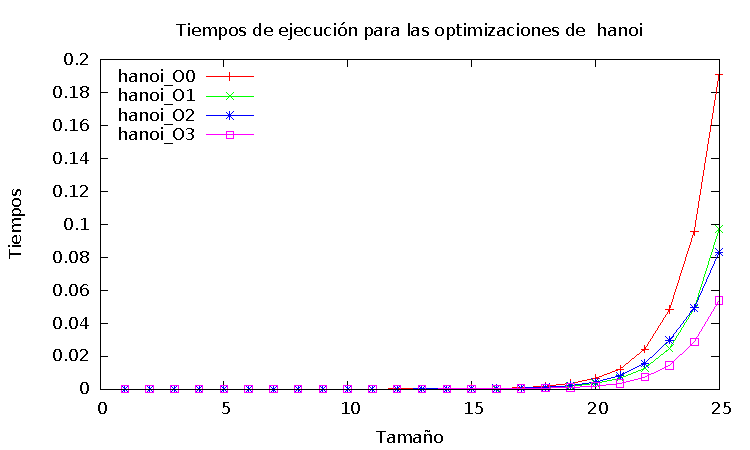
\includegraphics[width=13cm]{img/hanoi_optim_g.pdf} \centering
	\caption{Optimización Hanói}\end{figure}

\end{document}
